% Created 2023-04-14 Fri 20:28
% Intended LaTeX compiler: pdflatex
\documentclass[14pt,a4paper]{extarticle}
                \usepackage{blindtext}
    \usepackage[skip=12pt plus1pt, indent=30pt]{parskip}
    \usepackage{geometry}
    \geometry{
      a4paper,
      total={166mm,227mm},
      left= 29mm,
      right=29mm,
      top=32mm,
      bottom=32mm
      }
    \usepackage[utf8]{inputenc}
    \usepackage[T1]{fontenc}
    \usepackage{fixltx2e}
    \usepackage{graphicx}
    \usepackage{longtable}
    \usepackage{float}
    \usepackage{wrapfig}
    \usepackage{rotating}
    \usepackage[normalem]{ulem}
    \usepackage{amsmath}
    \usepackage{textcomp}
    \usepackage{marvosym}
    \usepackage{wasysym}
    \usepackage{amssymb}
    \usepackage{hyperref}
    \usepackage{mathpazo}
    \usepackage{color}
    \usepackage{enumerate}
    \usepackage{sectsty}    
    \definecolor{astral}{RGB}{46,116,181}
    \definecolor{bg}{rgb}{0.95,0.95,0.95}
    \definecolor{bg1}{rgb}{0.9,0.9,0.9}
    \definecolor{schrift}{RGB}{0,73,114}
    \tolerance=1000
                    
    \linespread{1.2}
    \hypersetup{pdfborder=0 0 0}
\author{vijay panchal}
\date{\today}
\title{}
\hypersetup{
 pdfauthor={vijay panchal},
 pdftitle={},
 pdfkeywords={},
 pdfsubject={},
 pdfcreator={Emacs 27.1 (Org mode 9.3)}, 
 pdflang={English}}
\begin{document}

\topskip0pt
\vspace*{\fill}
\normalsize
\noindent\rule{\linewidth}{.7ex}
\begin{flushright}
\begin{huge}\color{schrift}Function Generator using OpAmp\end{huge}\\
\vspace{.5cm} \large \textit{This project showcases DIY Function generator with 
satisfactory range and accuracy}\\
\vspace{1cm} \textbf{Ved \textsc{Rudani}, 64}\\
\vspace{0.1cm} \textbf{Vijay \textsc{Panchal}, 65}\\
\end{flushright}
\noindent\rule{\linewidth}{.7ex}


\vspace{2cm}
\begin{center}
    
\includegraphics[width=2in]{extras/logo_em.png} \\
    \vspace*{\stretch{1}}
    \Large Semester 2 Project \\
    \vspace*{\stretch{2}}
   \large Mentor: \textbf{Mr. D. B. \textsc{Patel}}\\
    \large Head of Department: \textbf{Dr. P. N. \textsc{Gajjar}}\\
    \vspace*{\stretch{1}}
    \large {Gujarat University}\\
    \large \today
  \end{center}
\vspace*{\fill}
\pagenumbering{roman} 
\setcounter{page}{1}
\pagebreak



\topskip0pt
\vspace*{\fill}
\begin{center}
\colorbox{bg1}{ \begin{minipage}{.95\textwidth}\centering \vspace{1.5cm} \Large \textbf{Abstract}\\
\begin{minipage}{0.8\textwidth} \vspace{.8cm} \normalsize Function generator are useful tools in academia and industries. Mostly they are avalaible in market. In this project we are trying to understand and study simple frequency generators with use of OpAmp. We usec generic OpAmp Ic LM741, which is single package and easy to understand with benefit of extensive acedemic experince. \vspace{1.5cm} \end{minipage}
\end{minipage}}
\end{center}
\vspace*{\fill}
\pagebreak

\topskip0pt
\vspace*{\fill}
\begin{center}
\begin{huge}
Acknowledgement\\
\end{huge}
\end{center}
\vspace{2cm}
\begin{large}
We would like to thank to the our Head of Department
- Dr. P. N. Gajjar sir for their faith in us and
supporting us in everyway. Special thanks to our
respected mentor Dr. D. B. Patel sir for their support,
encouragement and supervision in every step of this
project. We also thank to all our respected professors
for their support to complete this project successfully.\\
We would also like to thank scientists and authors on
whom work we build our work.\\
We are also grateful of our classmates for their help
and support for this project work. We heartly
appreciate their contribution and thank them too.\\
\end{large}

\vspace*{\fill}
\pagebreak


\renewcommand*\contentsname{Table Of Contents}
\tableofcontents
\pagebreak
\pagenumbering{arabic} 
\setcounter{page}{1}
\section{Introduction}
\label{sec:org4fef661}




Function generator is circuit which generates periodic function with predictable frequencies with respect to time. Here, we will study only mono frequency generator but it can also generate superposed functions. Signals from Function generator comes in many forms but mostly it is either sinusoidal or square wave. We will generate sinusoidal, square and triangle wave as output. 

We used basic circuits with few modification as our need. With use of IC LM741 we used OpAmp in our circuit.

For Sinusoidal wave we used Wein Bridge circuit, which is easy to understand and impliment. Also, wein bridge circuit is quite less noice compare to it's compitition RC phase shift Oscillator, which have more component than Wein bridge and more complicated to understand. For Square wave we used standard astable multivibrator cicuit, with little modification. Lastly, Triangle wave can be made from just attaching Integrator to our square wave output with some regulation.

Now, each circuit ( this wave form generator) has different block, basically we divided whole circuit in there block. Main work for us is to combine all of this. We wandered across CMOS families, BJTs but finally we sattled into physical swith which is coupled for power transmission and also for output change.\cite{gayakwad2012op}

\section{Blocks}
\label{sec:org2b09f8f}



As told in introduction each circuit is in their blocks. First block for sine wave which is nothing but wien bridge circuit, second is sqaure which is astable multivibrator, third for triangular wave which integrator attached to second block (square wave block).


\begin{figure}[htbp]
\centering
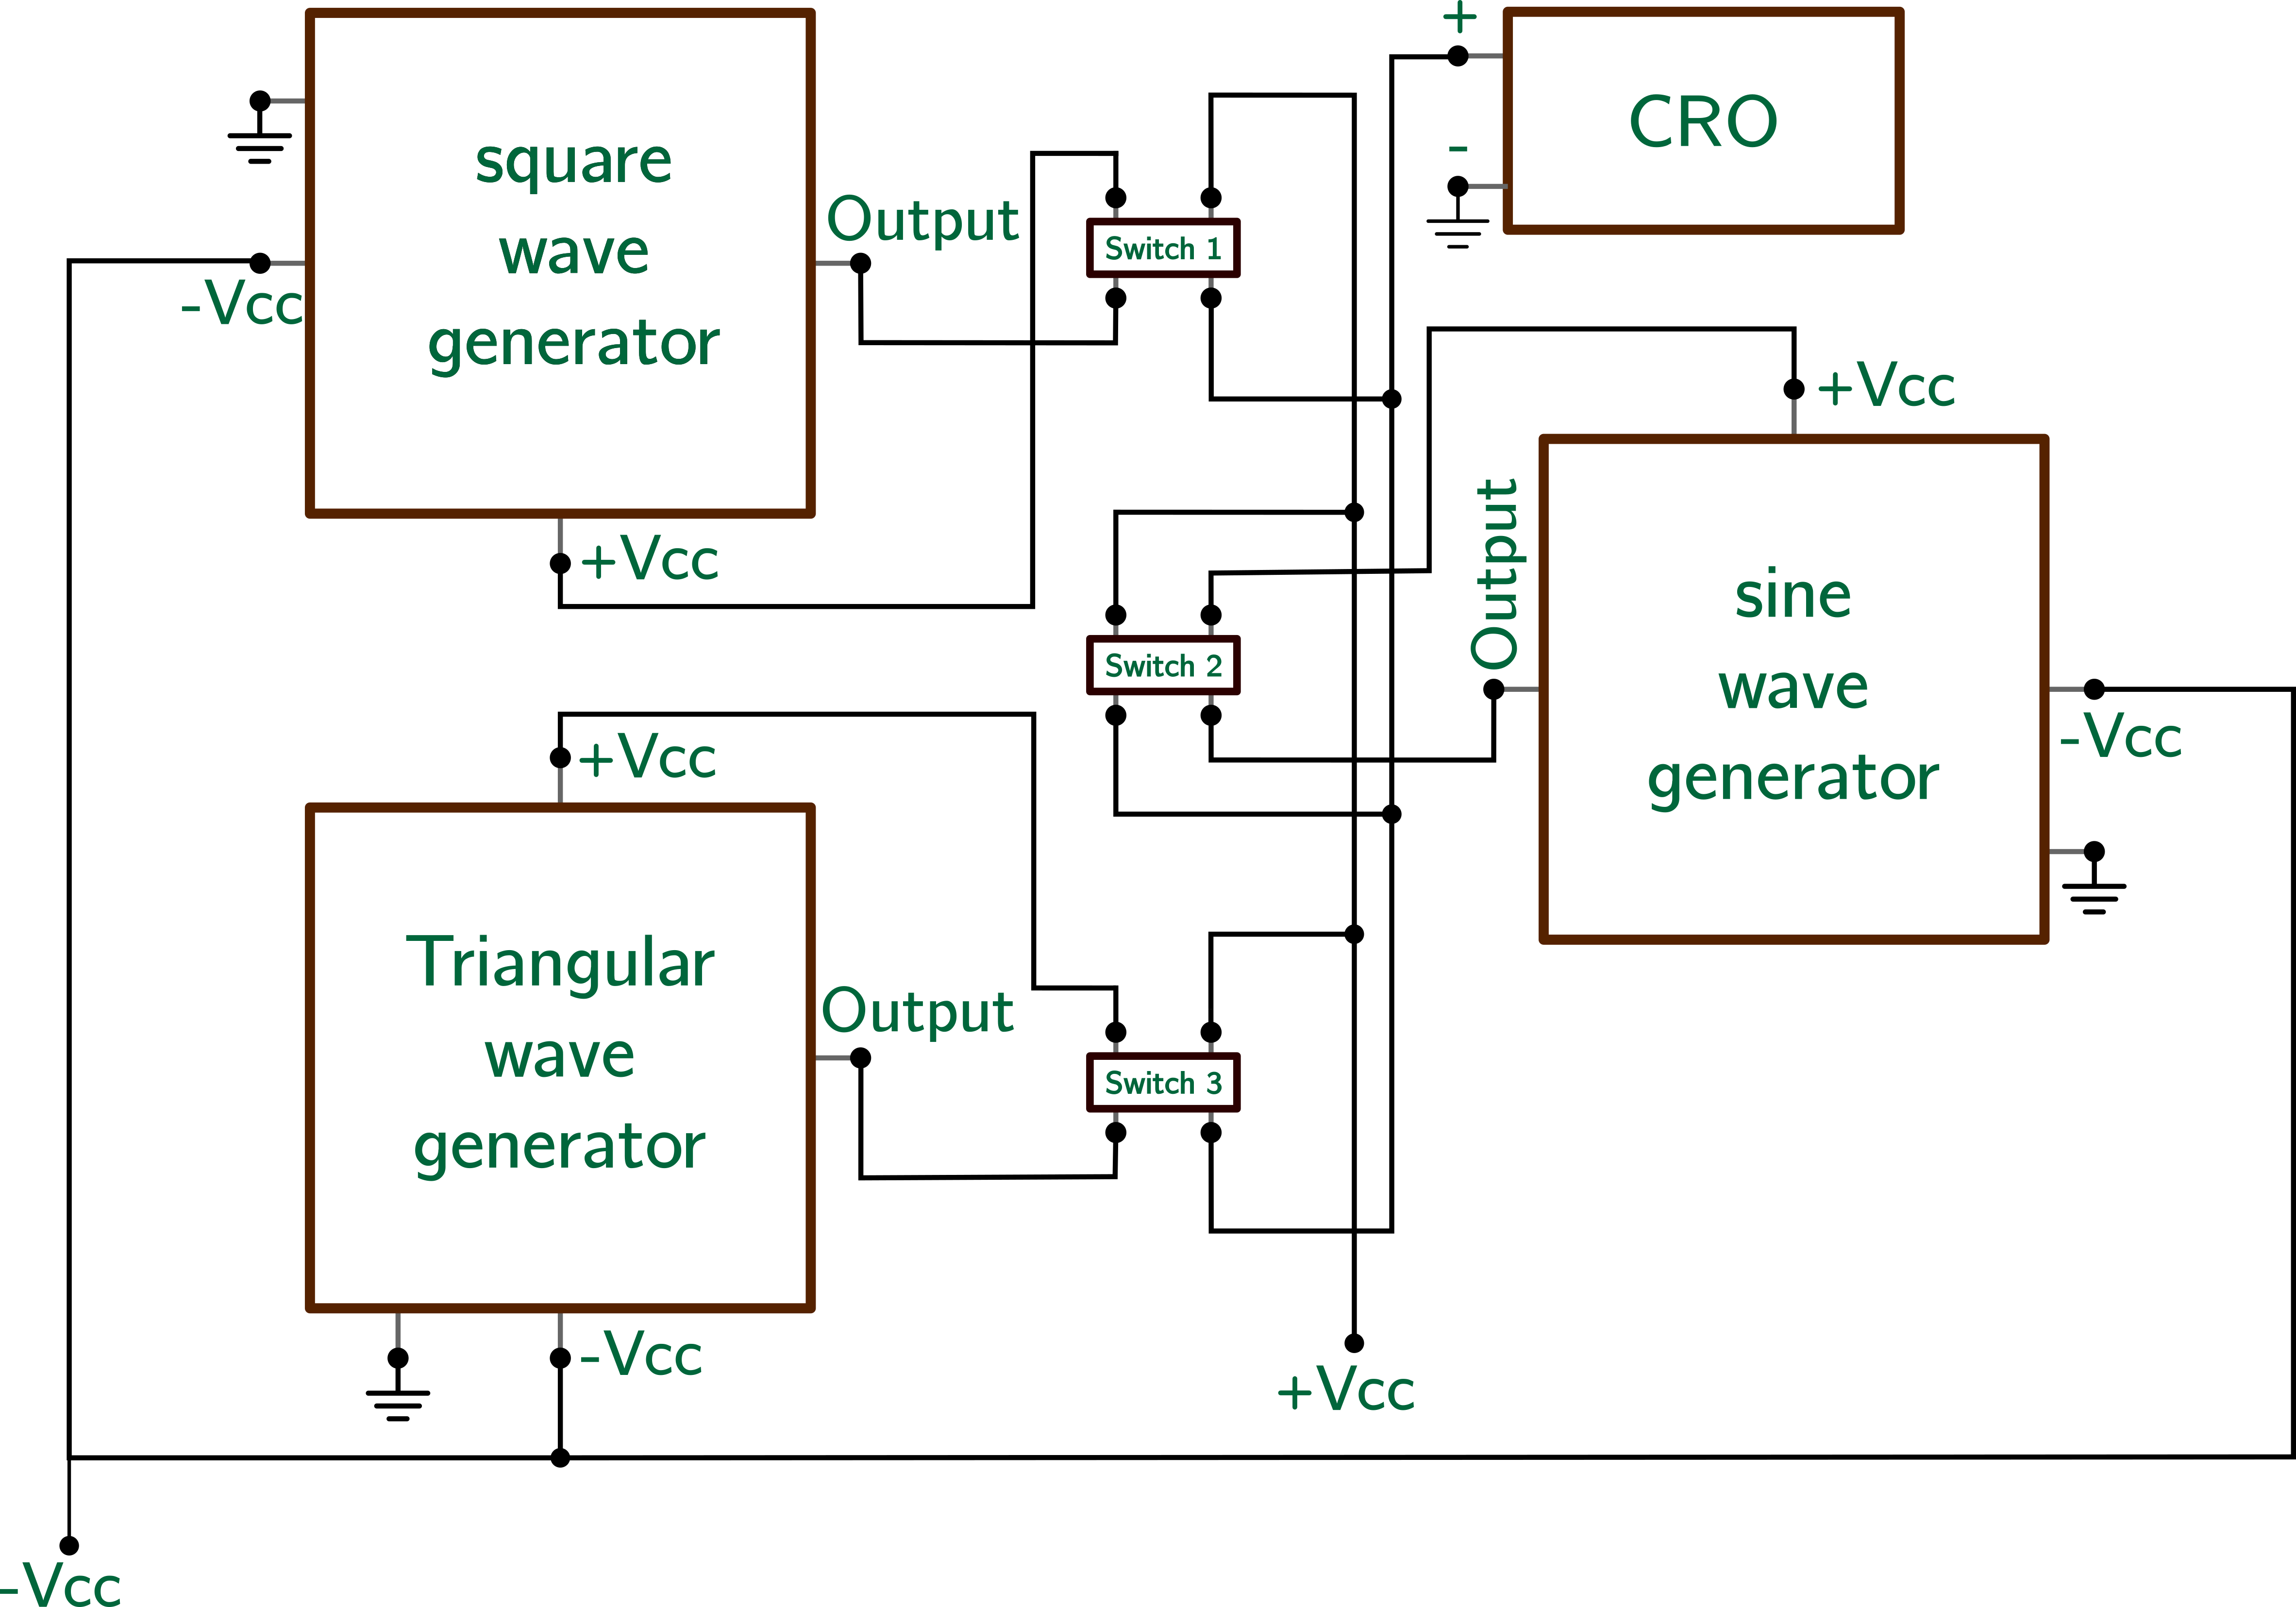
\includegraphics[width=.95\textwidth]{imgs/blocks.png}
\caption{\label{fig:org0f0169c}Block diagram of our function generator}
\end{figure}


\subsection{Block 1: Sine wave generator}
\label{sec:org4b2de51}


In first block, we have basic circuit of wein bridge. You can see in figure 1. In center we have OpAmp (IC LM741). This is amplifier with RC component attached with input and output. Here, at one end there is RC parallel component and at other end series RC component. 


\begin{figure}[ht]
    \centering
    \label{sine}
    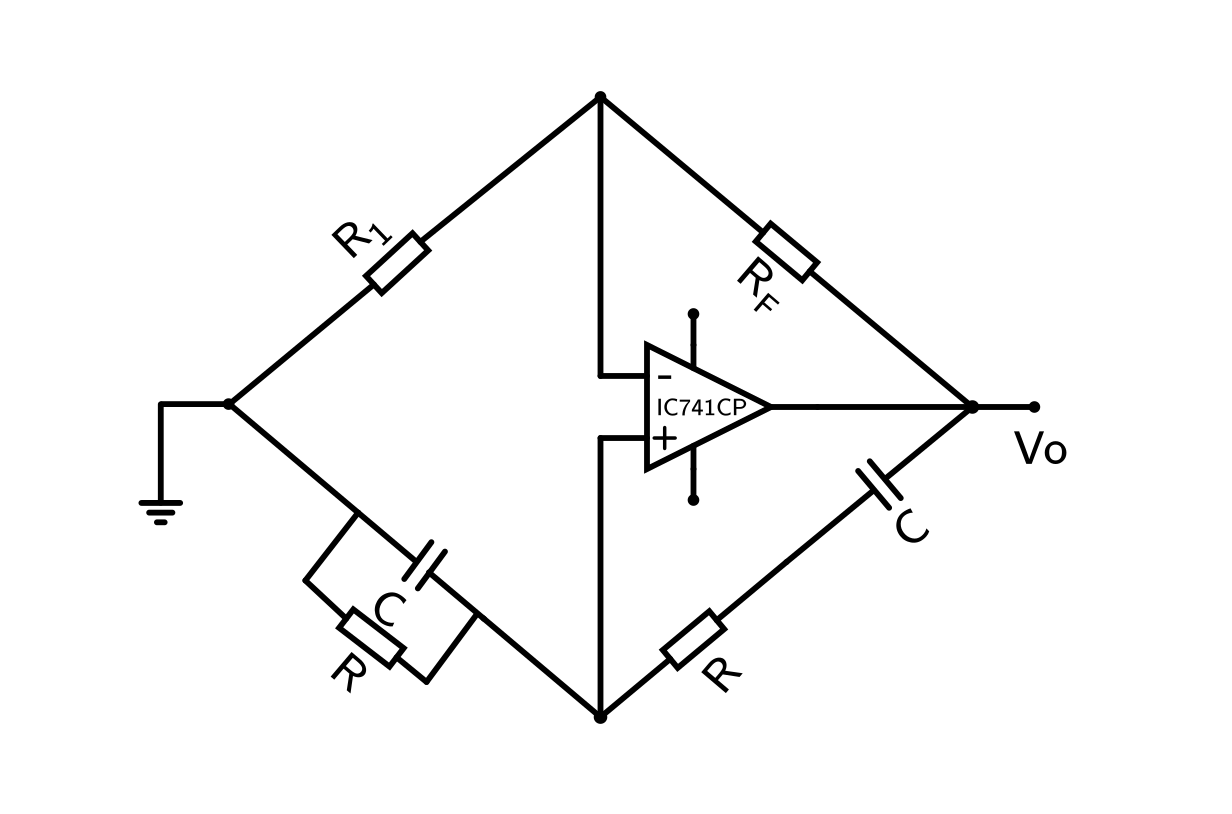
\includegraphics[width=0.7\textwidth]{imgs/sine.png}
    \caption{Wein bridge circuit}
\end{figure}

Here, frequency is given by, 

\begin{equation}
\label{eq:orge48d5a7}
  f =\frac{1}{2 \pi RC}
\end{equation}

For sustaing oscilation gain must be 3 and for non inverting amplifier gain, 

\begin{equation}
\label{eq:orgf3838a2}
  A = 1+\frac{R_{F}}{R_{1}} = 3
\end{equation}

So, we get relation \(R_{F}=R_{1}\)

\begin{figure}[ht]
    \centering
    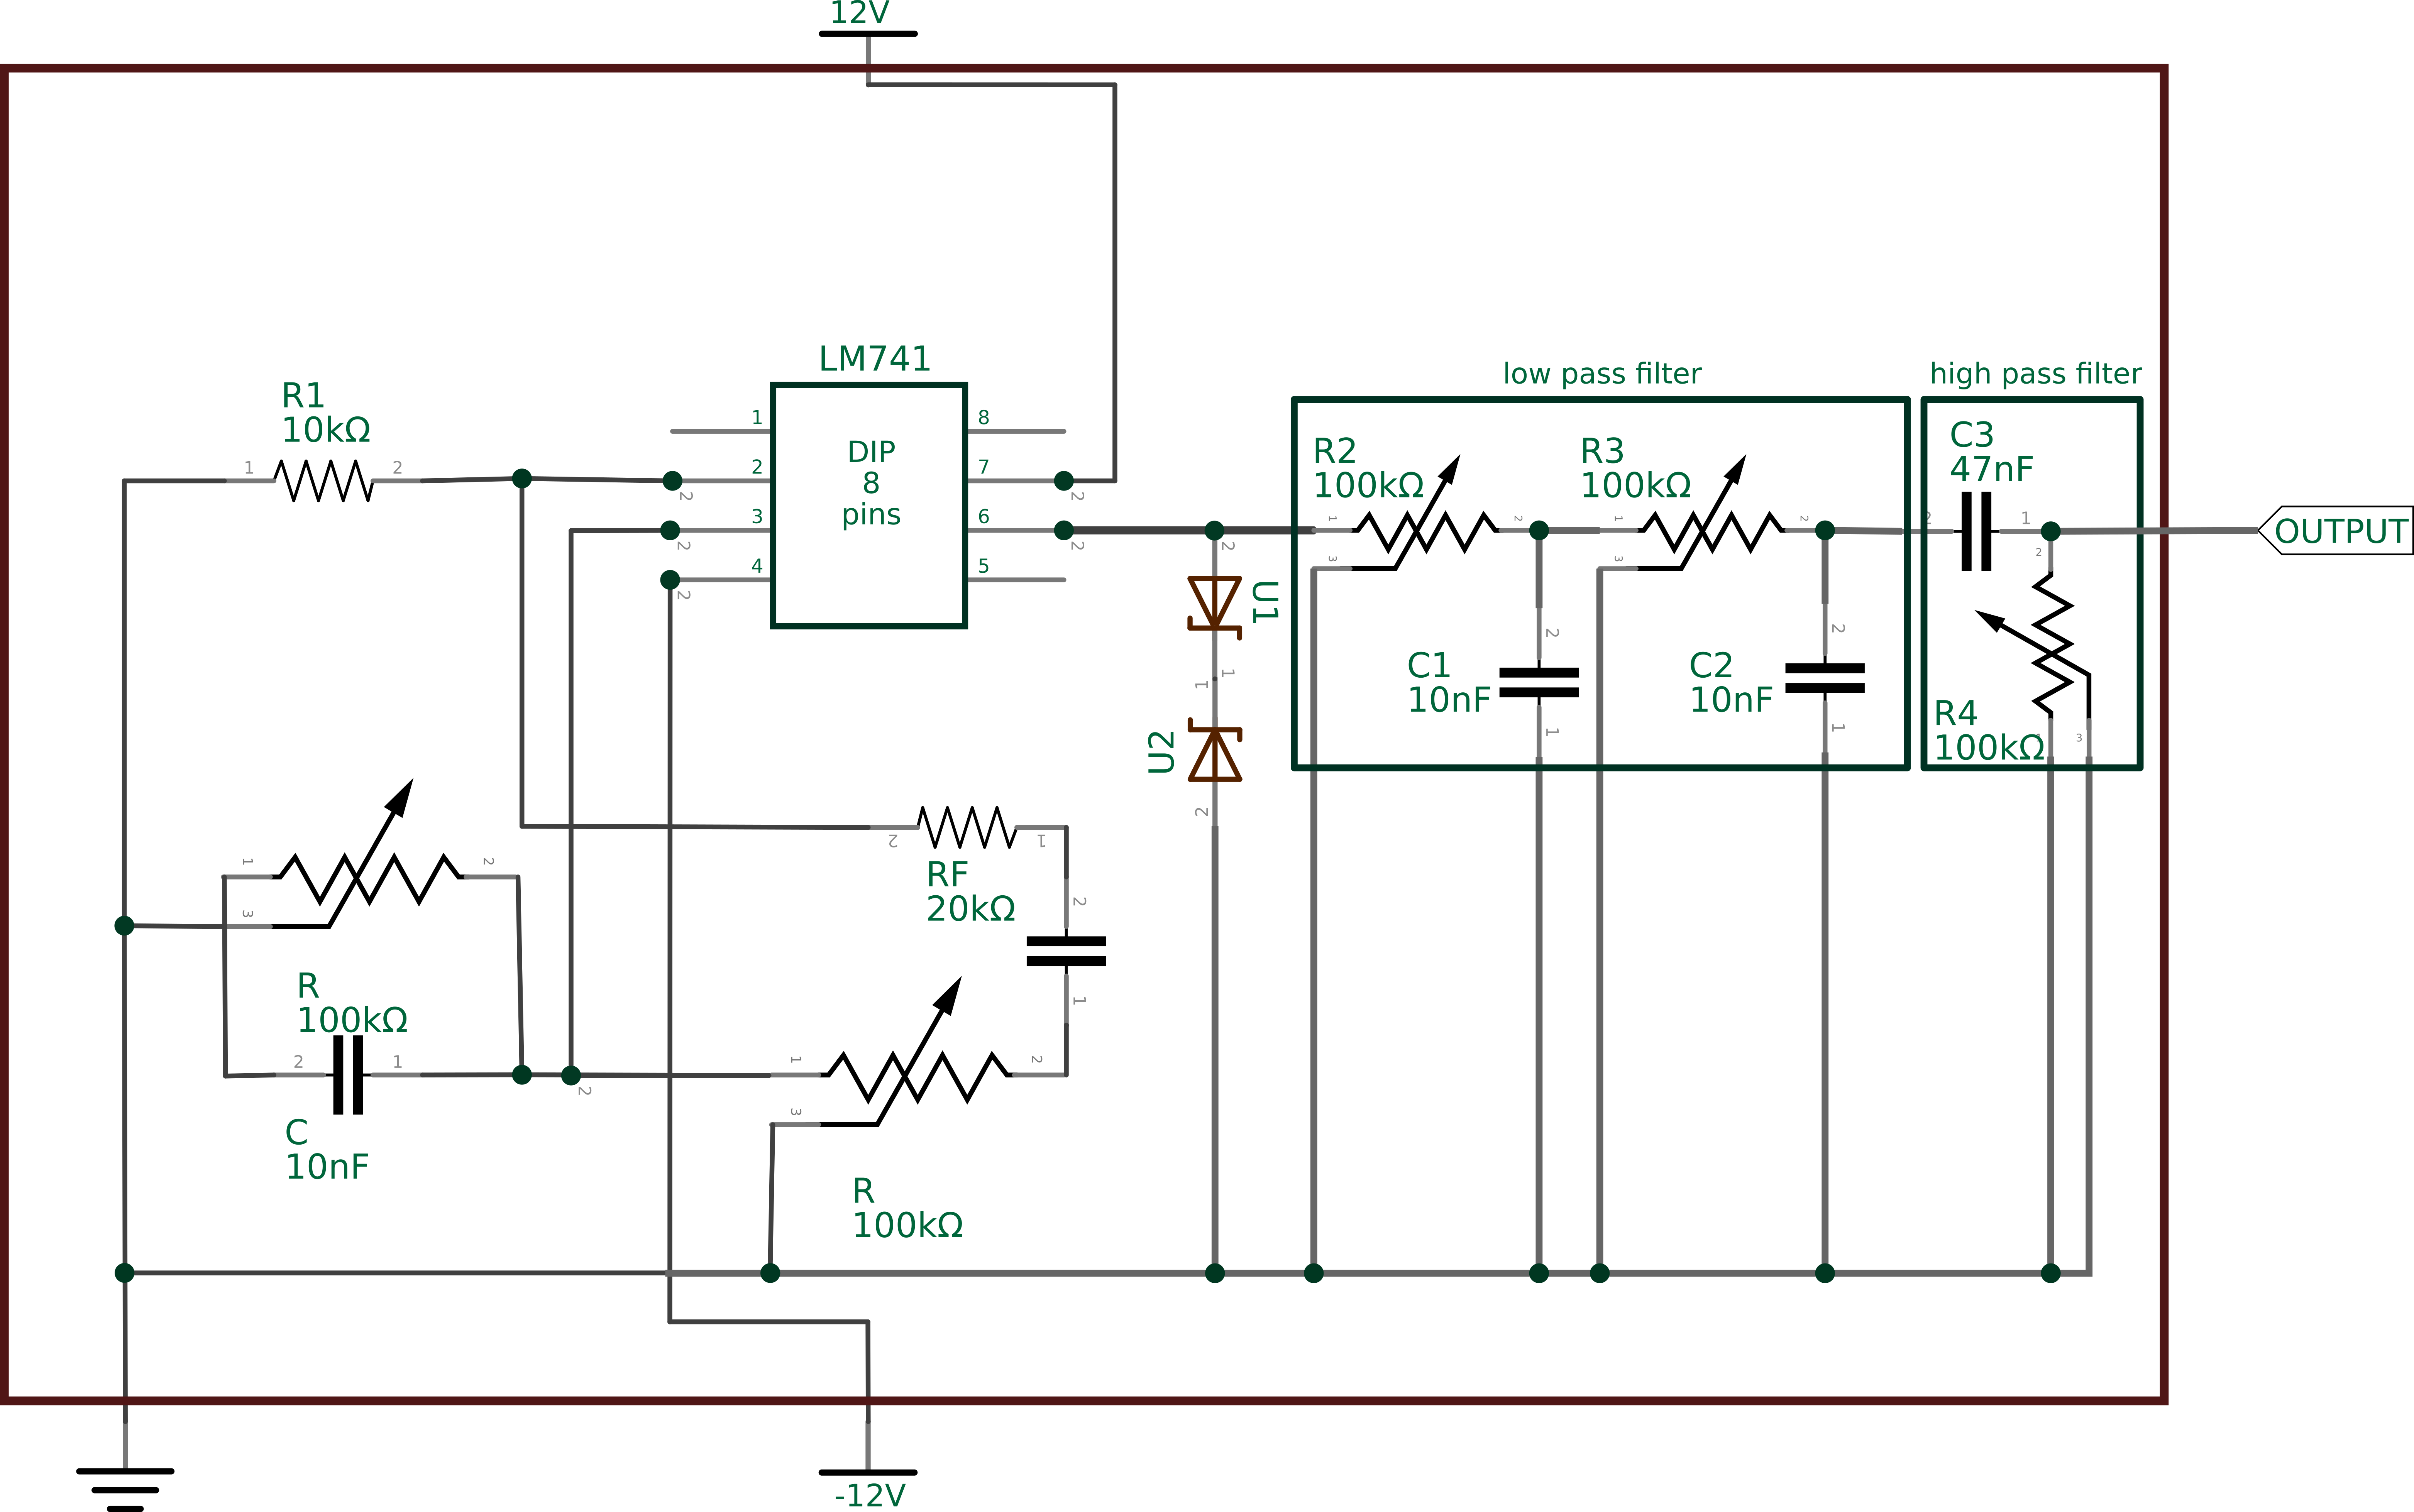
\includegraphics[width=0.9\textwidth]{imgs/sinereal.png}
    \caption{Our block 1, which consinst of IC741CP}
    \label{fig:realsine}
\end{figure}


Here, you can see our block circuit, at the end we attached two zener diode for regulation to the output. As you can see OpAmp in IC LM741 package. Power supply given from  4 and 7 to 12V and -12V. We chose \(R_{1}=12k\Omega\). By relation of \(R_{1}\) and \(R_{F}\), we got \(R_{F}=24k\Omega\).

For frequency range we used Potential with max range of \(100k\Omega\). So, lowest and maximum frequency whould be (with constant capacitance at \(50nF\)),

\begin{equation*}
\label{eq:orgbc48f63}
  f_{min} = \frac{1}{2\pi\times100k\times 10n} \approx 159 hz
\end{equation*}

\begin{equation*}
\label{eq:org998ea2c}
  f_{max} = \frac{1}{2\pi\times100\times 10n} \approx 159k hz
\end{equation*}

So, frequency range would be \(159 hz\) to \(159k hz\)

\subsection{Tuning sine wave generator}
\label{sec:org8f71875}

The output of sine wave generator can be little noisy. This will be reasonable as we will see it's working. Any sine wave generator will work as frequency extractor from DC or any AC levels. Since, Row signals have superposed waves in nearly all the spectrum, one have to rely on different filters and component which can attenuate desire frequency and theoretically minimize every other frequency. 


In wien bridge, this is principle is mostly exploited. We have two RC components, one in series make low pass filter and secondly there is parallel component which work as high pass filter. In \textbf{\textbf{figure}} there is highlighted areas of both filters. Here, it is quite straight forward see that low pass will block higher frequency and high pass will vice versa. So, if we set both filter such that combination will give us some band (quite narrow band in fact). Center of this frequencies will cut off frequency of both filters. When wien bridge balances than this band of frequency will be resonated and give final output.

\subsubsection{Series RC components in Wien bridge}
\label{sec:org9053ffe}
Series RC component which works as low pass filter have this type of phenomenan, total \(V_{in}\) and \(V_{out}\) will be proportional to the to total reactance. With voltage divider low, 


\begin{equation*}
\frac{V_o}{V_i}= \frac{X_c}{R+X_c}
\end{equation*}

Where, \(X_c\) is reactance of capacitor valued as \(\frac{-j}{wC}\). So,

\begin{equation*}
\frac{V_o}{V_i}=\left(\frac{1}{1+w^2R^2C^2}\right)^{\frac{1}{2}}
\end{equation*}

If we take \(w_0\) as breakpoint or curoff point for our RC component than \(w_0=\frac{1}{RC}\). Here RC is time constant. 

Graph of low pass shown in figure \ref{fig:filters}a. Where we can see frequency equals to \(w=w_0\) at some point. Also, notice that even though we have cutoff frequency at \(w_0\), there is enough frequencies around \(w_0\). Basically filters always have some noise which does not filtered. Here, if you use higher order filter than this slope of voltage to frequency would be slightly higher. With sufficiently high order filter you can make abrupt change in frequency domain, but this comes with it's consequences. With higher order filters other noises dominates since we will have too much components. We will use second order filter here, which is quite balance in accuracy and component noise.


\begin{figure}[h]
\centering
\begin{tabular}{cc}
    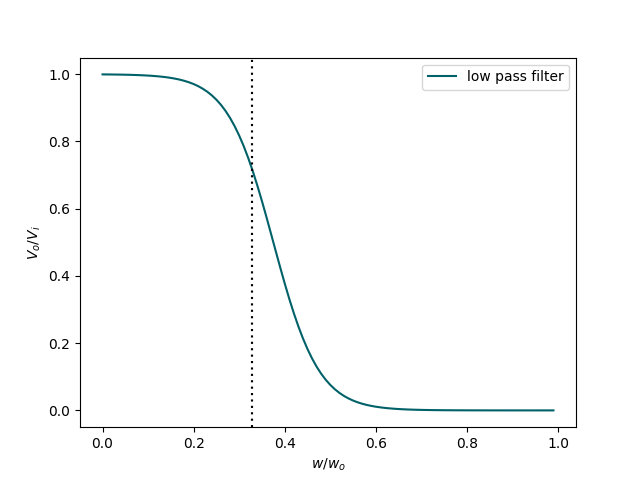
\includegraphics[width=0.5\linewidth]{imgs/low.png}&
    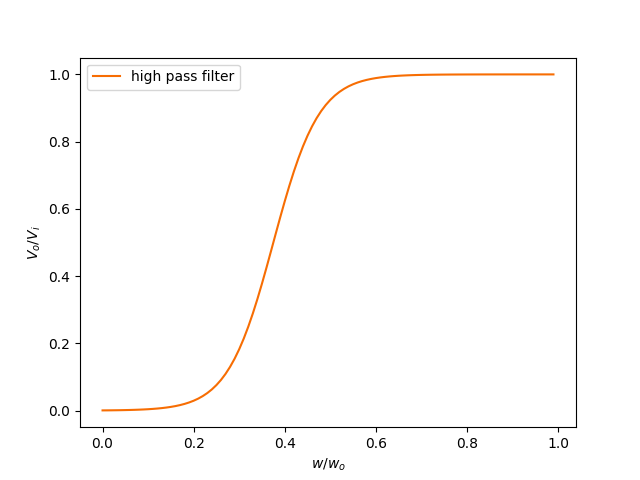
\includegraphics[width=0.5\linewidth]{imgs/high.png}
\end{tabular}
\vspace{0.2cm}
\centering
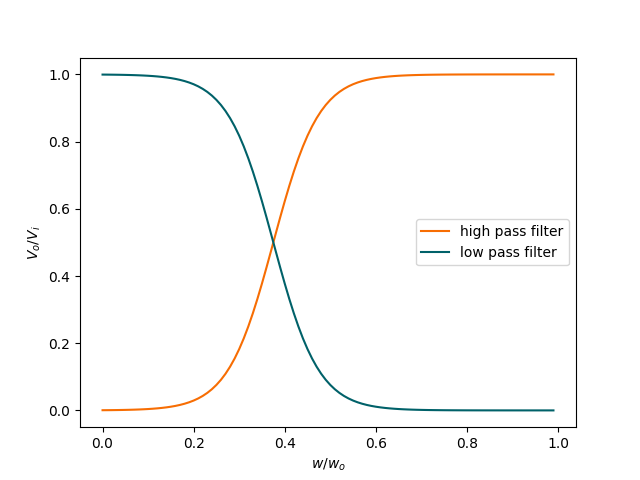
\includegraphics[width=0.5\linewidth]{imgs/highlow.png}
\caption{here, we have a) low pass filter, b) high pass filter and c) combination of high and low pass fiter}
\label{fig:filters}
\end{figure}


\subsubsection{Parallel RC components in Wien bridge}
\label{sec:org38bb3b7}
Similarly to that of series RC components, we can define high pass filter as parallel RC component. In parallel circuit when frequency increases reactance decreases and total reactance decreases. So, consequently higher frequency pass and lower frequency will not. Reactance of high pass filter would be following, 


\begin{equation*}
\frac{V_o}{V_i}= \frac{R}{R+X_c}
\end{equation*}

Again, \(X_c\) is capacitance reactance and valued at \(-frac{-j}{wC}\)

\begin{equation*}
\frac{V_o}{V_i}=\left(\frac{R^2}{R^2+\frac{1}{w^2C^2}}\right)^{\frac{1}{2}}
\end{equation*}

This relationship is shown in figure \ref{fig:filters}b. With cutoff frequency at \(w_0\). As we can see here also noise of unwanted frequency range are here. 


\subsubsection{Total signal and Error terms}
\label{sec:orgc45a2a4}
In wien bridge we have both the low pass and high pass filters. So, total response of that shown in figure \ref{fig:filters}c. Here, we have gain frequencies in range between cutoff frequency. Since, this range amplify in non inverting amplifier and feedback. This frequency will resonant and becomes our output signal. From now on, we will say \(w_0\) as resonant frequency. Final output in our theoretical studies will be this resonant frequency. Practically this frequency is observed with error frequencies.

Error terms in here will be in following cases. \emph{1) since we have band, we get many frequency output from the band, which is quite distorted in itself.} and \emph{2) here working of filters are note up to expectation and we have noise from whole spectrum of frequency.} This is quite headache, unfortunately we have both the cases in our experiment. 


\subsubsection{Fourier analysis of Output signal}
\label{sec:org01b21a4}

We can minimize this errors by using Fourier analysis of output signal. As one can say that DC level is made of superposed infinite number of waves with different wavelengths,

\begin{equation*}
DC_{level}= \sum_{n}^{\infty}(a_n\cos(w_nt)+b_n\sin(w_nt))
\end{equation*}

Here, \(a_n\) and \(b_n\) are coefficients of Fourier series. What wein bridge does is extract desire frequency from DC level. 


In our experiment we got distorted sine wave which means their is higher frequencies in effect. Also after some values of Potentiometer, there is just square signal. Another distortion occur was from lower frequencies manly \(\appro 50Hz\) and around \(300Hz\), which are making signal less stable and sometimes dominates resonant frequency. 


For higher frequency, we got idea to put low pass filter around value of resonant frequency that would bring signal to more on resonant frequency. This is can be seen in block diagram of sine wave from figure \ref{fig:realsine} and figure below \ref{fig:lowpass}. This should give us better results ad we intended.


\begin{figure}[h]
\centering
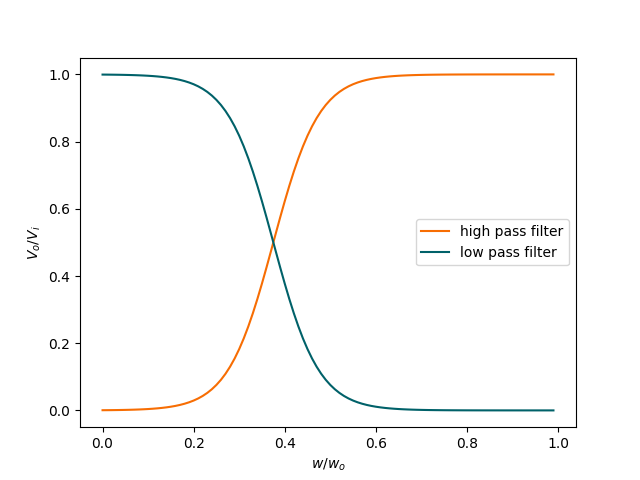
\includegraphics[width=0.5\linewidth]{imgs/highlow.png}
\caption{low pass filter at the output of our signal}
\label{fig:lowpass}
\end{figure}


For lower frequency, we have high pass filter, which eliminate those lower frequencies and stabilize our signal. This can be shown from block diagram figure \ref{fig:realsine} and figure \ref{fig:highpass}.


\begin{figure}[h]
\centering
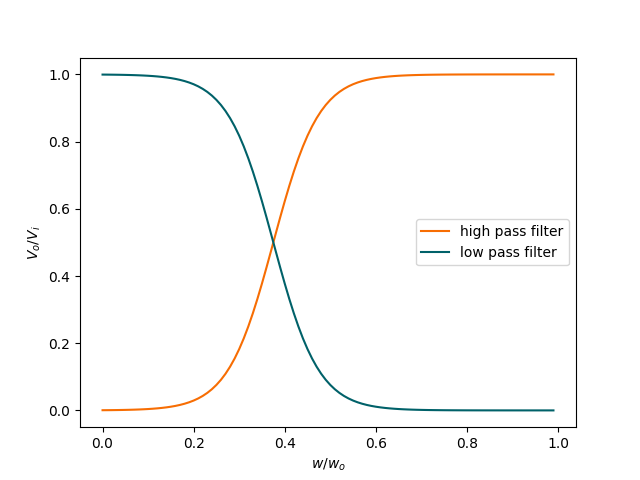
\includegraphics[width=0.5\linewidth]{imgs/highlow.png}
\caption{high pass filter at the output of our signal}
\label{fig:highpass}
\end{figure}

\begin{figure}[H]
\centering
\begin{tabular}{ccc}
    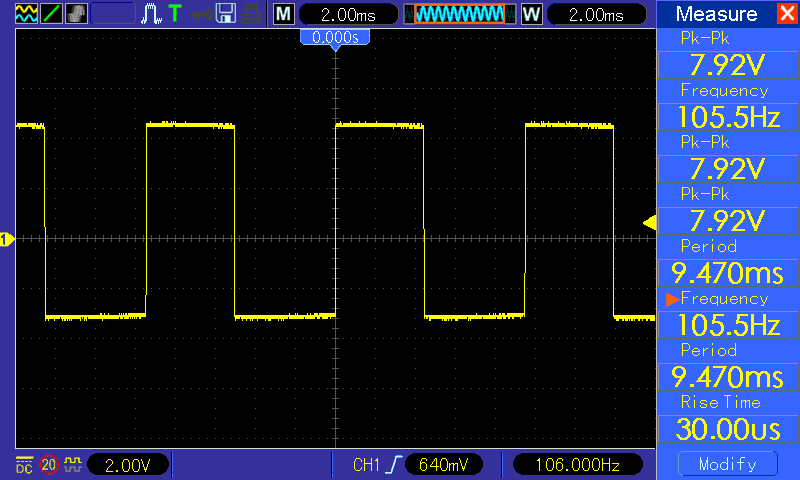
\includegraphics[width=0.32\linewidth]{imgs/square100.png}&
    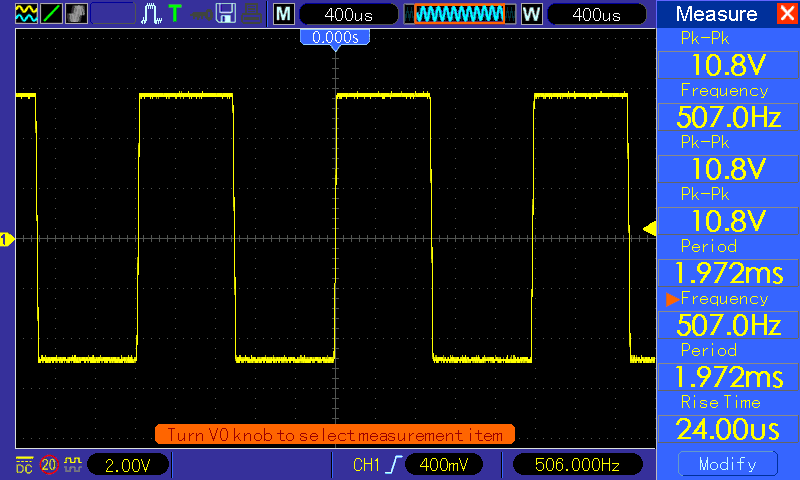
\includegraphics[width=0.32\linewidth]{imgs/square500.png}&
    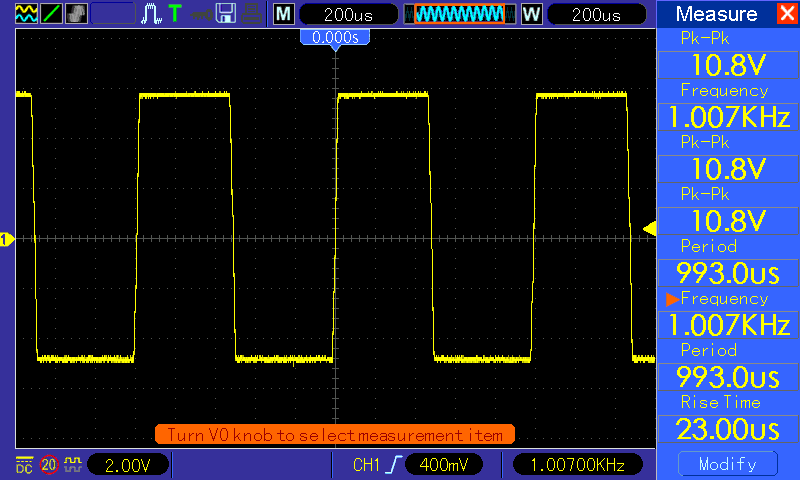
\includegraphics[width=0.32\linewidth]{imgs/square1k.png}\\
    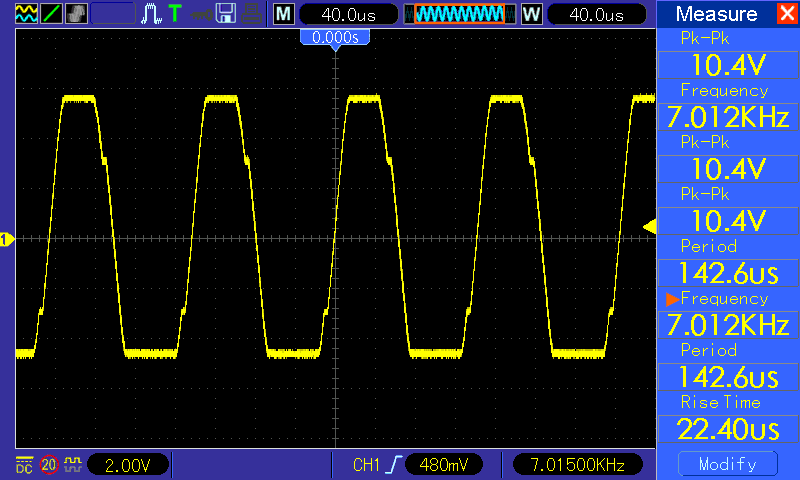
\includegraphics[width=0.32\linewidth]{imgs/square7k.png}&
    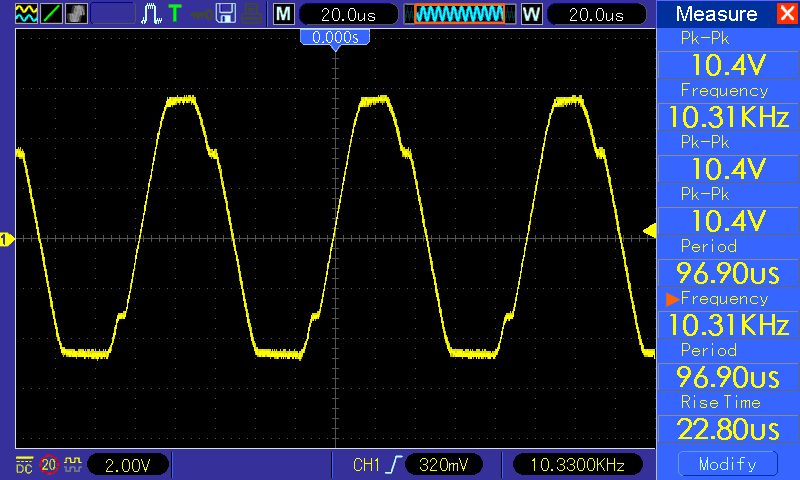
\includegraphics[width=0.32\linewidth]{imgs/square10k.png}&        
    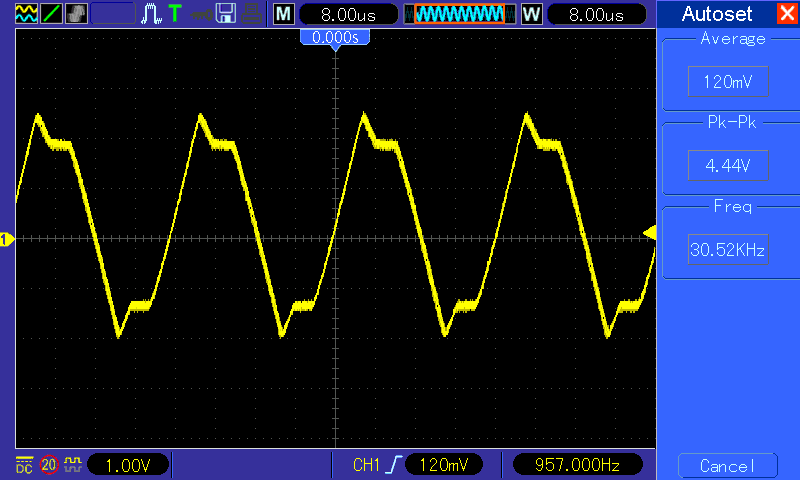
\includegraphics[width=0.32\linewidth]{imgs/square30k.png}\\
    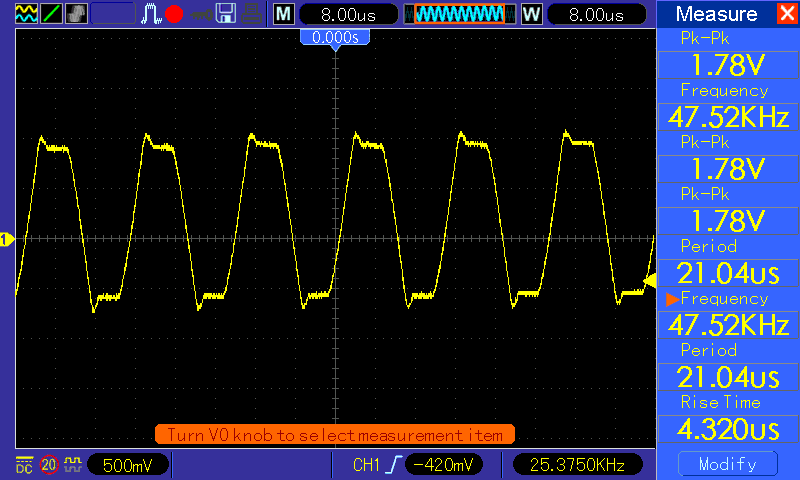
\includegraphics[width=0.32\linewidth]{imgs/square47k.png}&
    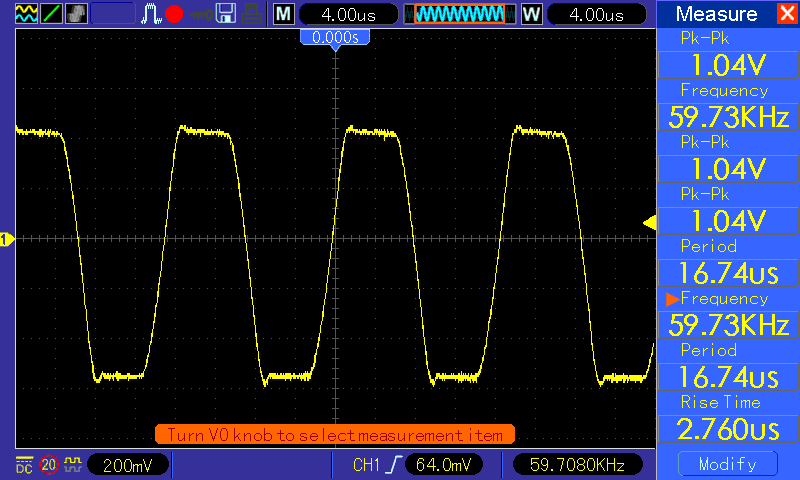
\includegraphics[width=0.32\linewidth]{imgs/square60k.png}&
    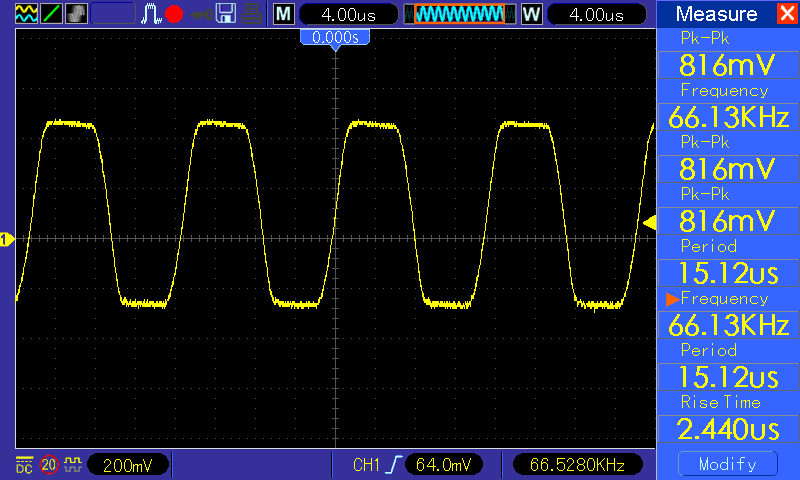
\includegraphics[width=0.32\linewidth]{imgs/square66k.png}
\end{tabular}
\vspace{0.2cm}
\caption{You can see all square wave outputs left to right respectevely 100Hz, 500Hz, 1kHz, 7kHz, 10kHz, 30kHz, 47kHz, 60kHz and 66kHz}
\label{fig:filters}
\end{figure}

\subsubsection{Output of sine wave after tuning}
\label{sec:org80422f9}
The output which we expected from our upper analysis at different frequency is shown below in figure \ref{fig:sineout}. The frequency range of sine wave output is given below in table. You should know that this \(V_{out}{p-p}\) is after applying all the filters and tuning. Original output is quite large in peak to peak voltage around 5 times big.

\begin{figure}[ht]
\centering
\begin{tabular}{ccc}
    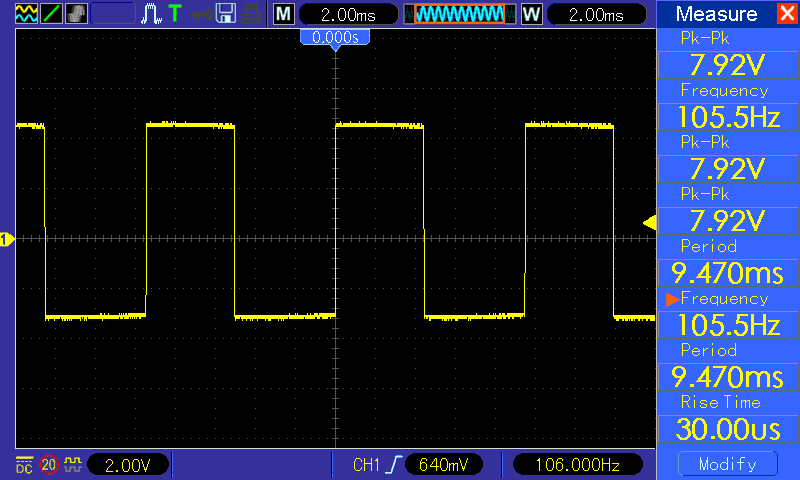
\includegraphics[width=0.33\linewidth]{imgs/square100.png}&
    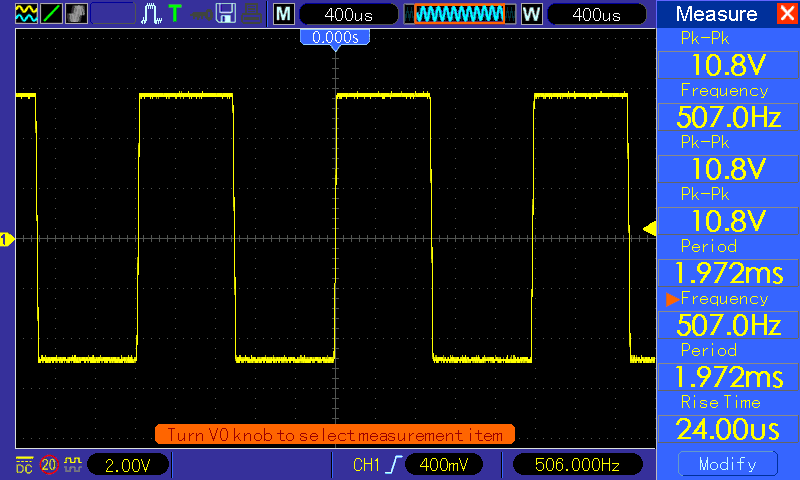
\includegraphics[width=0.33\linewidth]{imgs/square500.png}&
    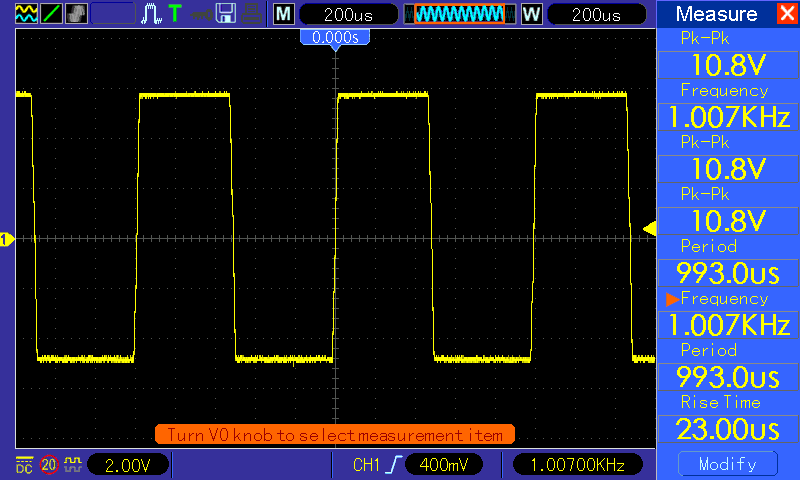
\includegraphics[width=0.33\linewidth]{imgs/square1k.png}\\
    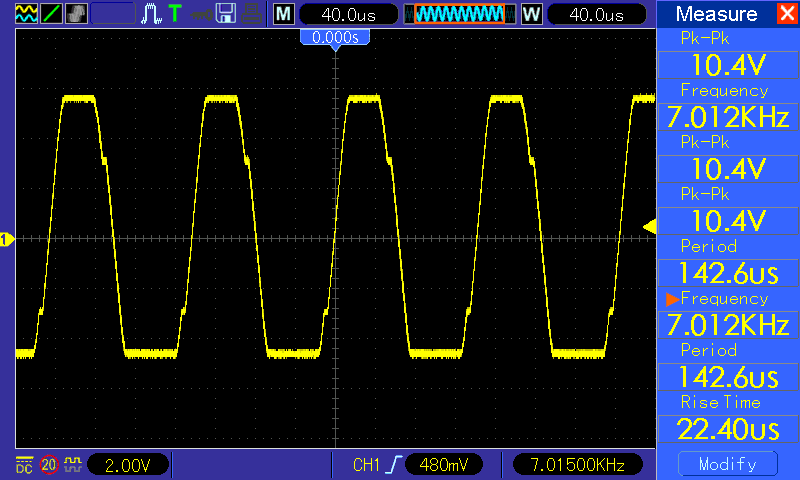
\includegraphics[width=0.33\linewidth]{imgs/square7k.png}&
    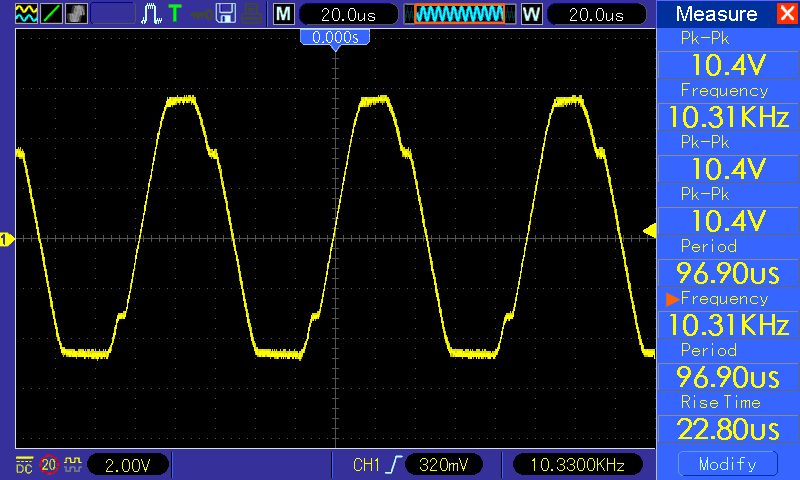
\includegraphics[width=0.33\linewidth]{imgs/square10k.png}&        
    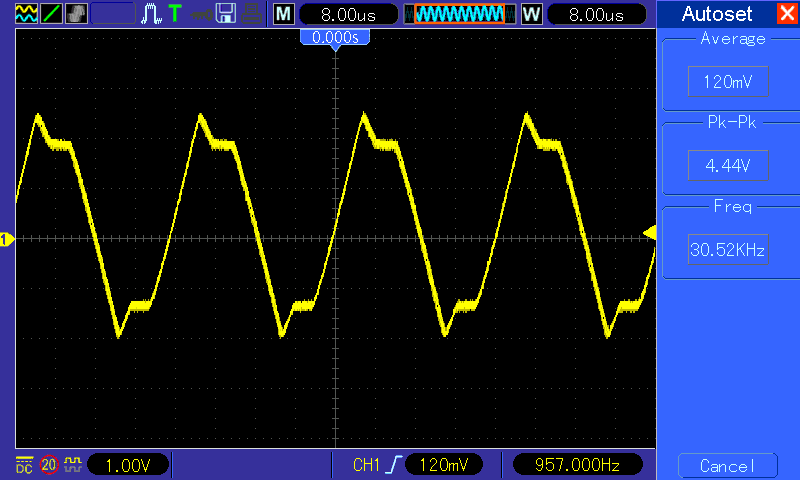
\includegraphics[width=0.33\linewidth]{imgs/square30k.png}\\
    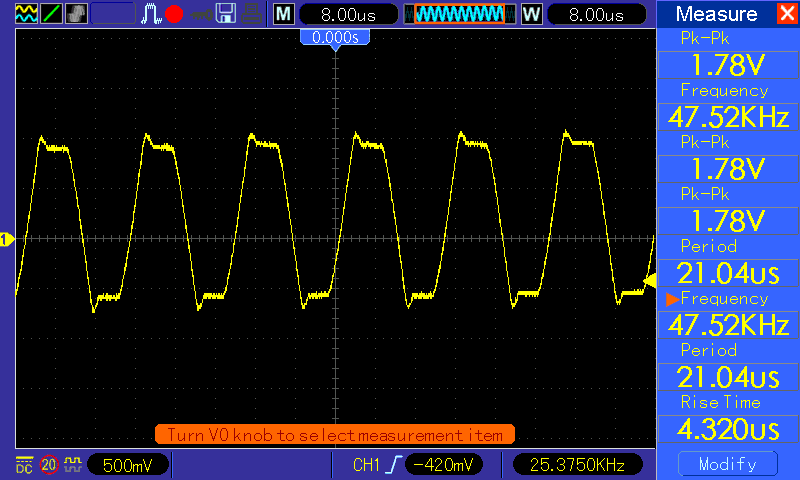
\includegraphics[width=0.33\linewidth]{imgs/square47k.png}&
    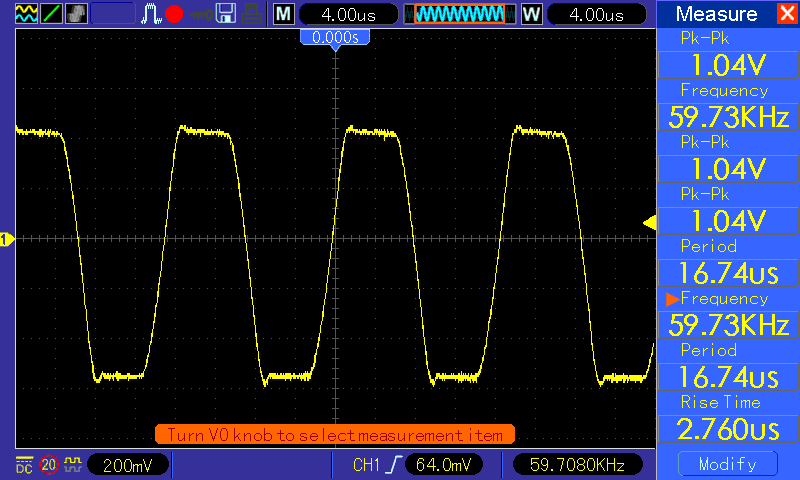
\includegraphics[width=0.33\linewidth]{imgs/square60k.png}&
    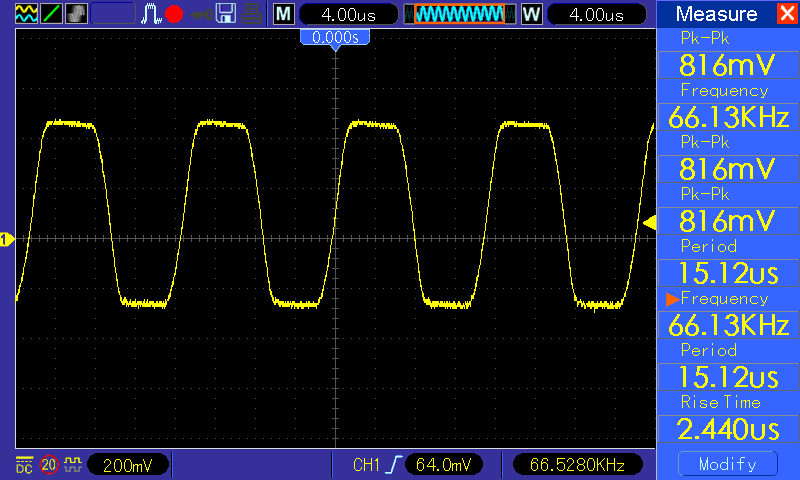
\includegraphics[width=0.33\linewidth]{imgs/square66k.png}
\end{tabular}
\vspace{0.2cm}
\caption{here, we have a) low pass filter, b) high pass filter and c) combination of high and low pass fiter}
\label{fig:filters}
\end{figure}










\subsection{Block 2: Square wave generator}
\label{sec:org6e42c7f}

As square wave generator we have basic astable multivibrator. This circuit works on scenario where output will have to stable state and it will swing between them, hence the name. When circuit is \(+V_{sat}\), we will have high signal output and when circuit is \(-V_{sat}\), we will have low signal output. So, we will have square wave as desired. The circuit for astable multivibrator is shown below.

\begin{figure}[H]
    \centering
    \label{square}
    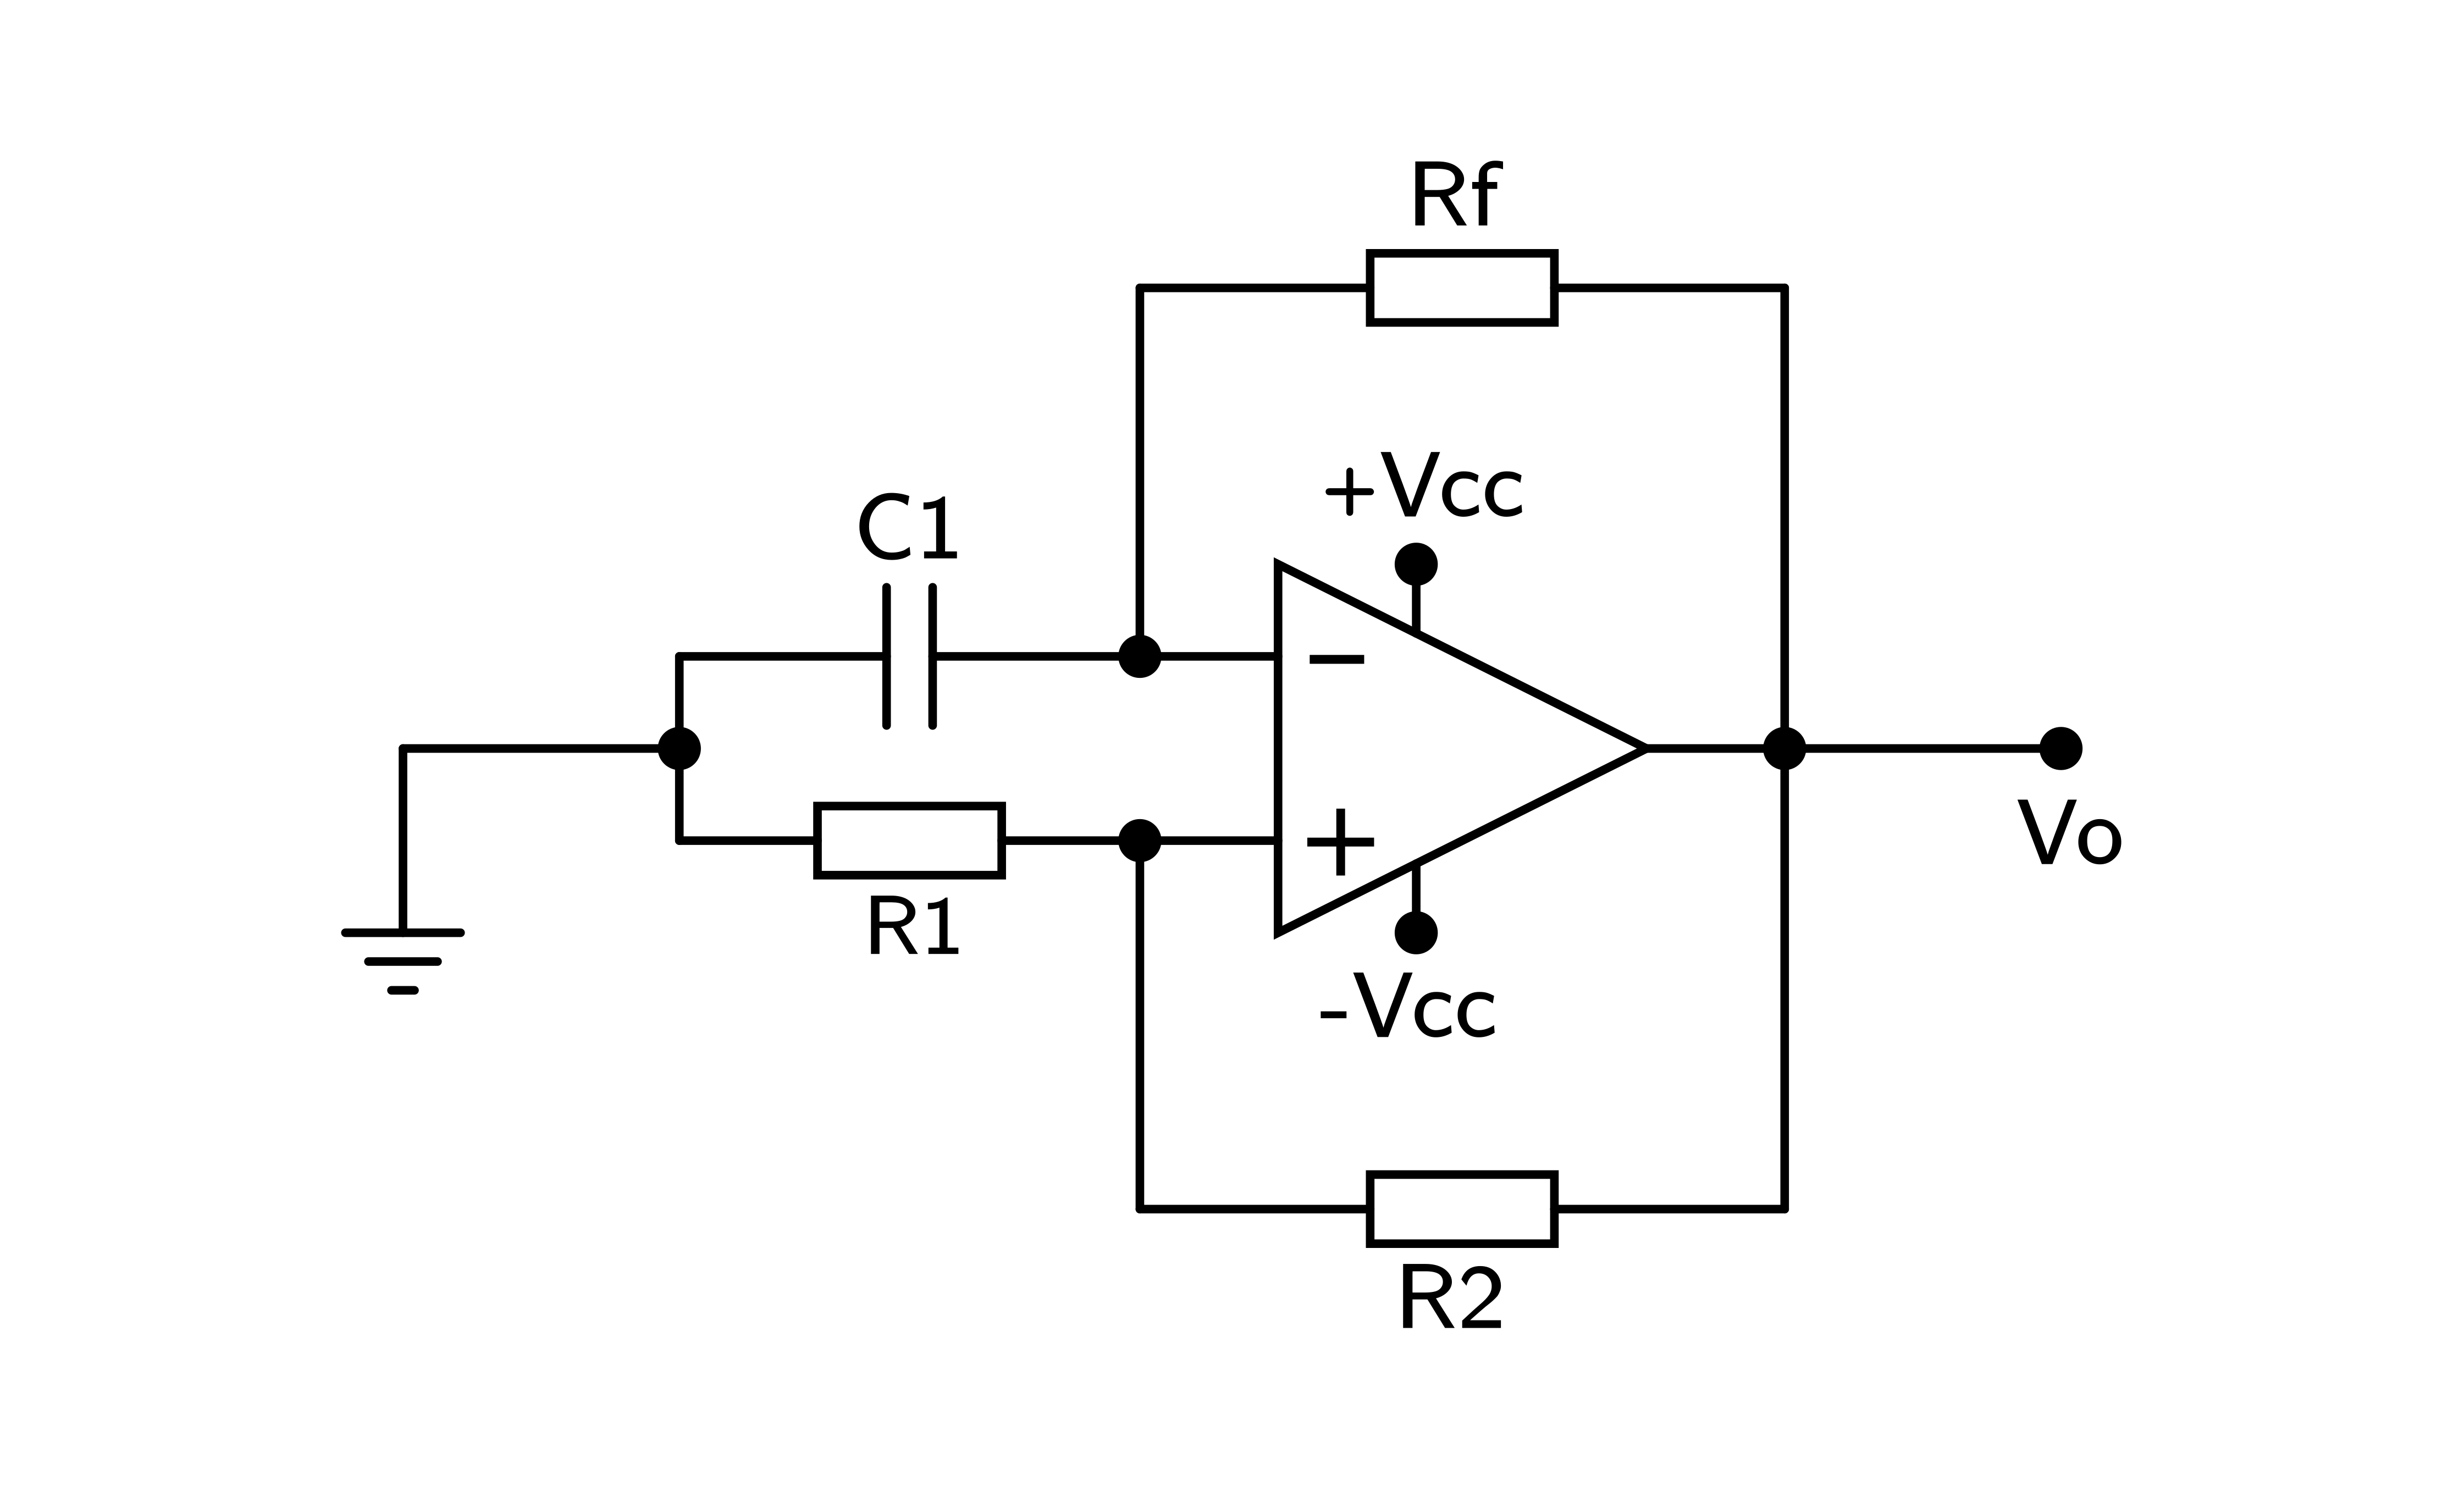
\includegraphics[width=0.65\textwidth]{imgs/square.png}
    \caption{astable multivibrator circuit}
\end{figure}


\begin{figure}[H]
    \centering
    \label{squarereal}
    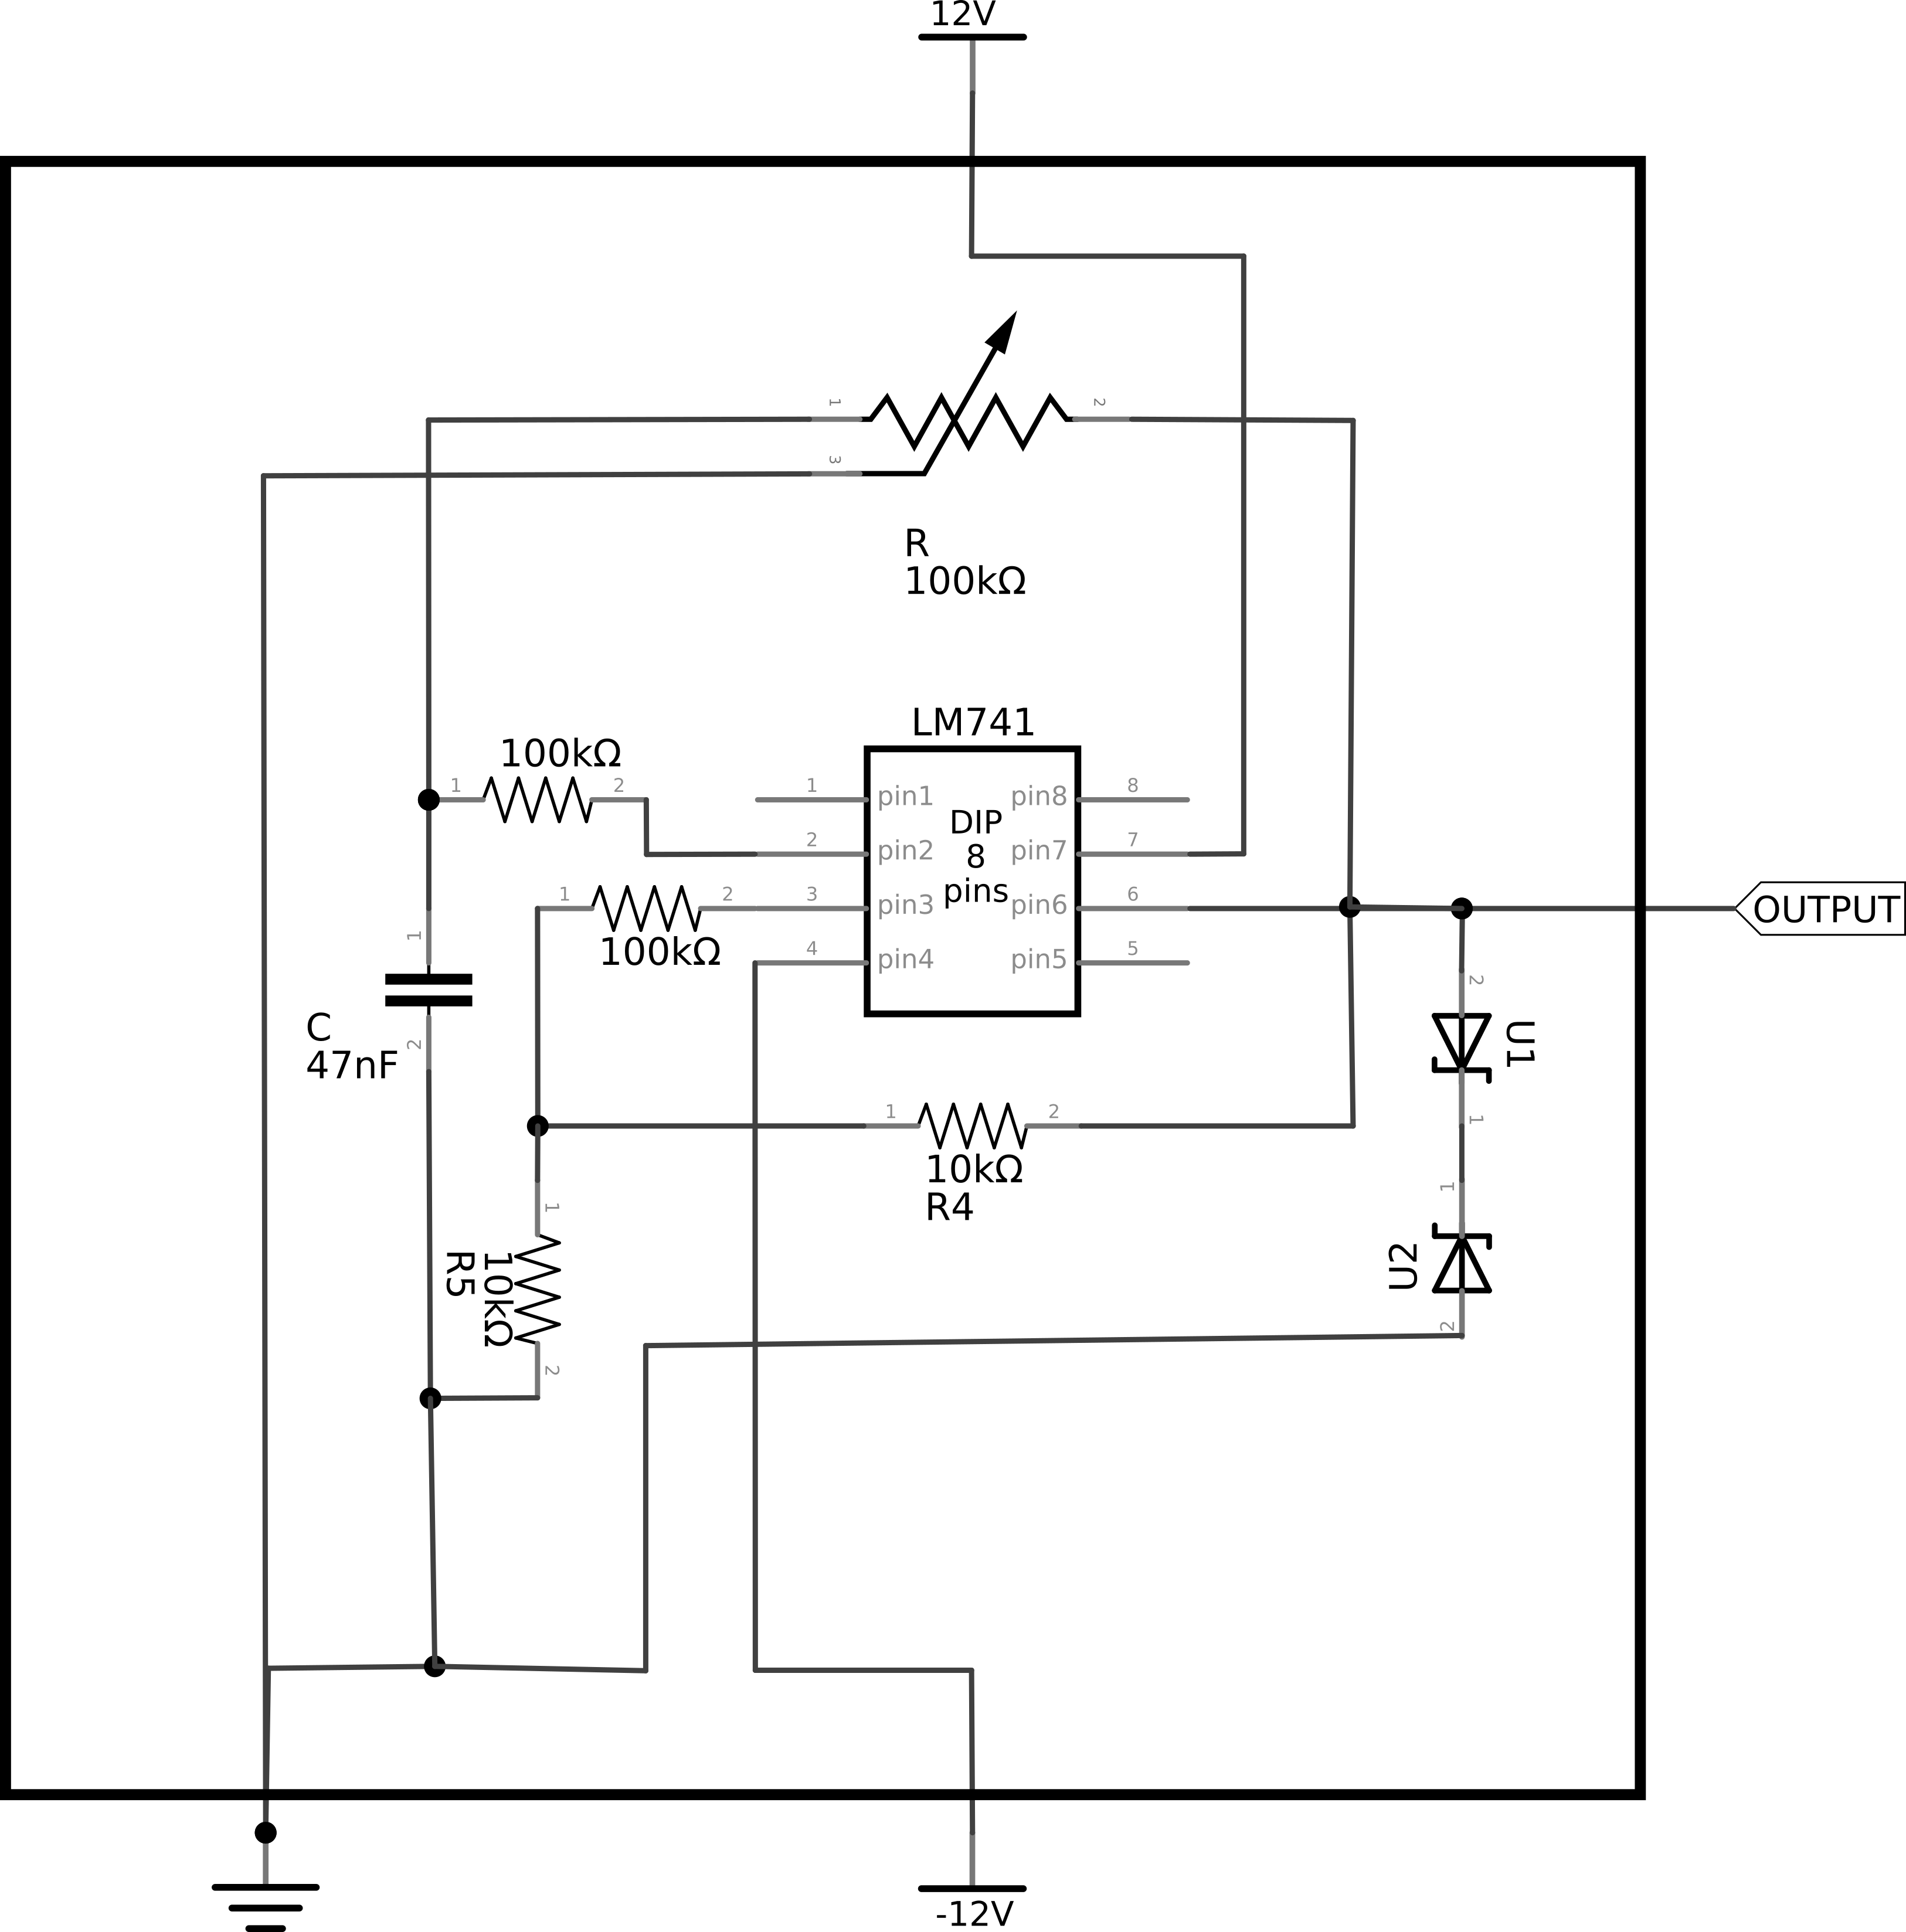
\includegraphics[width=0.75\textwidth]{imgs/squarereal.png}
    \caption{second block: square wave generator}
\end{figure}


Here, frequency would be, 

\begin{equation}
\label{eq:org6e99115}
  f =\frac{1}{2 RC ln(\frac{2R_{1}+R_{2}}{R_{2}})}
\end{equation}

If, we take \(R_{2}=1.16R_{1}\) then, 

\begin{equation}
\label{eq:org850789a}
  f =\frac{1}{2RC}
\end{equation}


Here, we took \(R_{1} = 10k\Omega\) and \(R_{2} = 11.6k\Omega\) such that \(\frac{R_{2}}{R_{1}}=1.16\). Also, you can see that we employed \(100k\Omega\) in input terminals for accurate and reliable signal.

Frequency range would be of (for constant capacitance at \(50nF\)),

\begin{equation*}
\label{eq:orgc58d777}
  f_{min} =\frac{1}{2\times 100k\times 50n} \approx 100 hz
\end{equation*}

\begin{equation*}
\label{eq:orgfae27d0}
  f_{max} =\frac{1}{2\times 100 \times 50n} \approx 100 khz
\end{equation*}


\subsection{Block 3: Triangluar Wave generator}
\label{sec:orgd345d61}

We basically extend block 2 with integrator circuit. Which would give triangular wave as intended. Here, this integrator circuit differs from basic circuit that \(100k\Omega\) as feedback resister is joined. Which would give better stability and accurate output. Circuit diagram is shown below,


\begin{figure}[H]
    \centering
    \label{triang}
    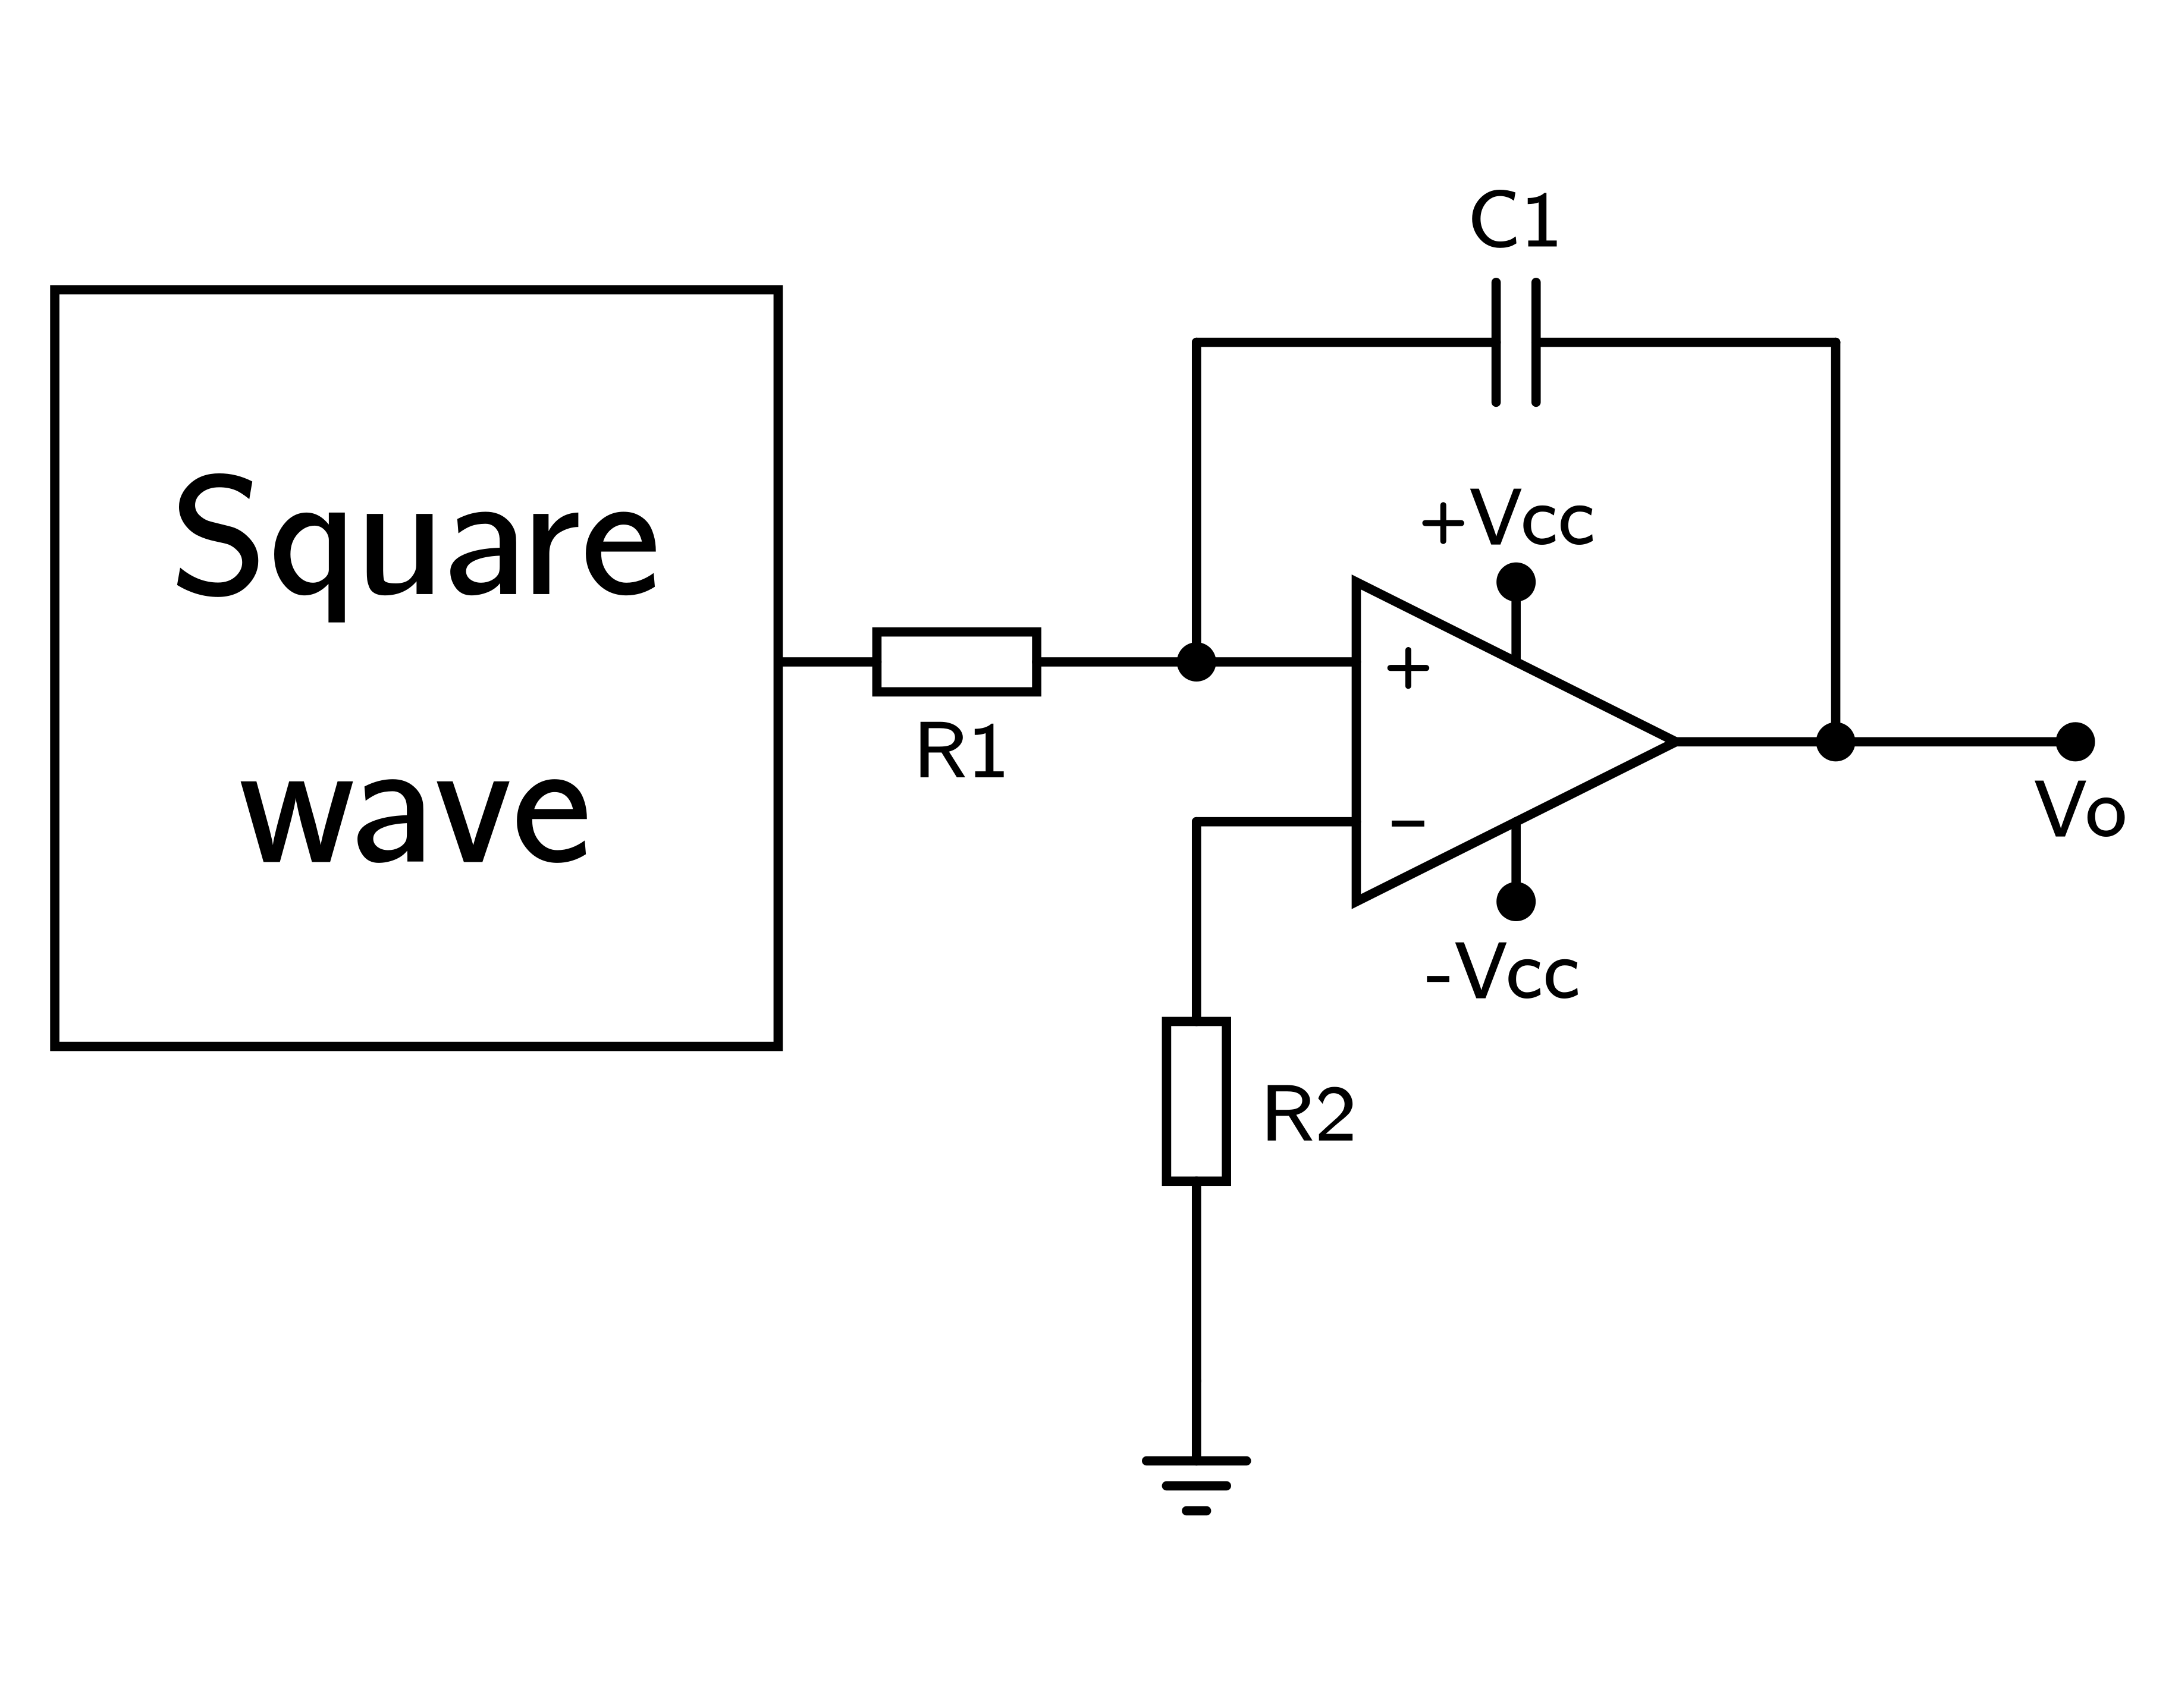
\includegraphics[width=0.5\textwidth]{imgs/triang.png}
    \caption{integrator circuit with square wave as input}
\end{figure}

\begin{figure}[H]
    \centering
    \label{tringularreal}
    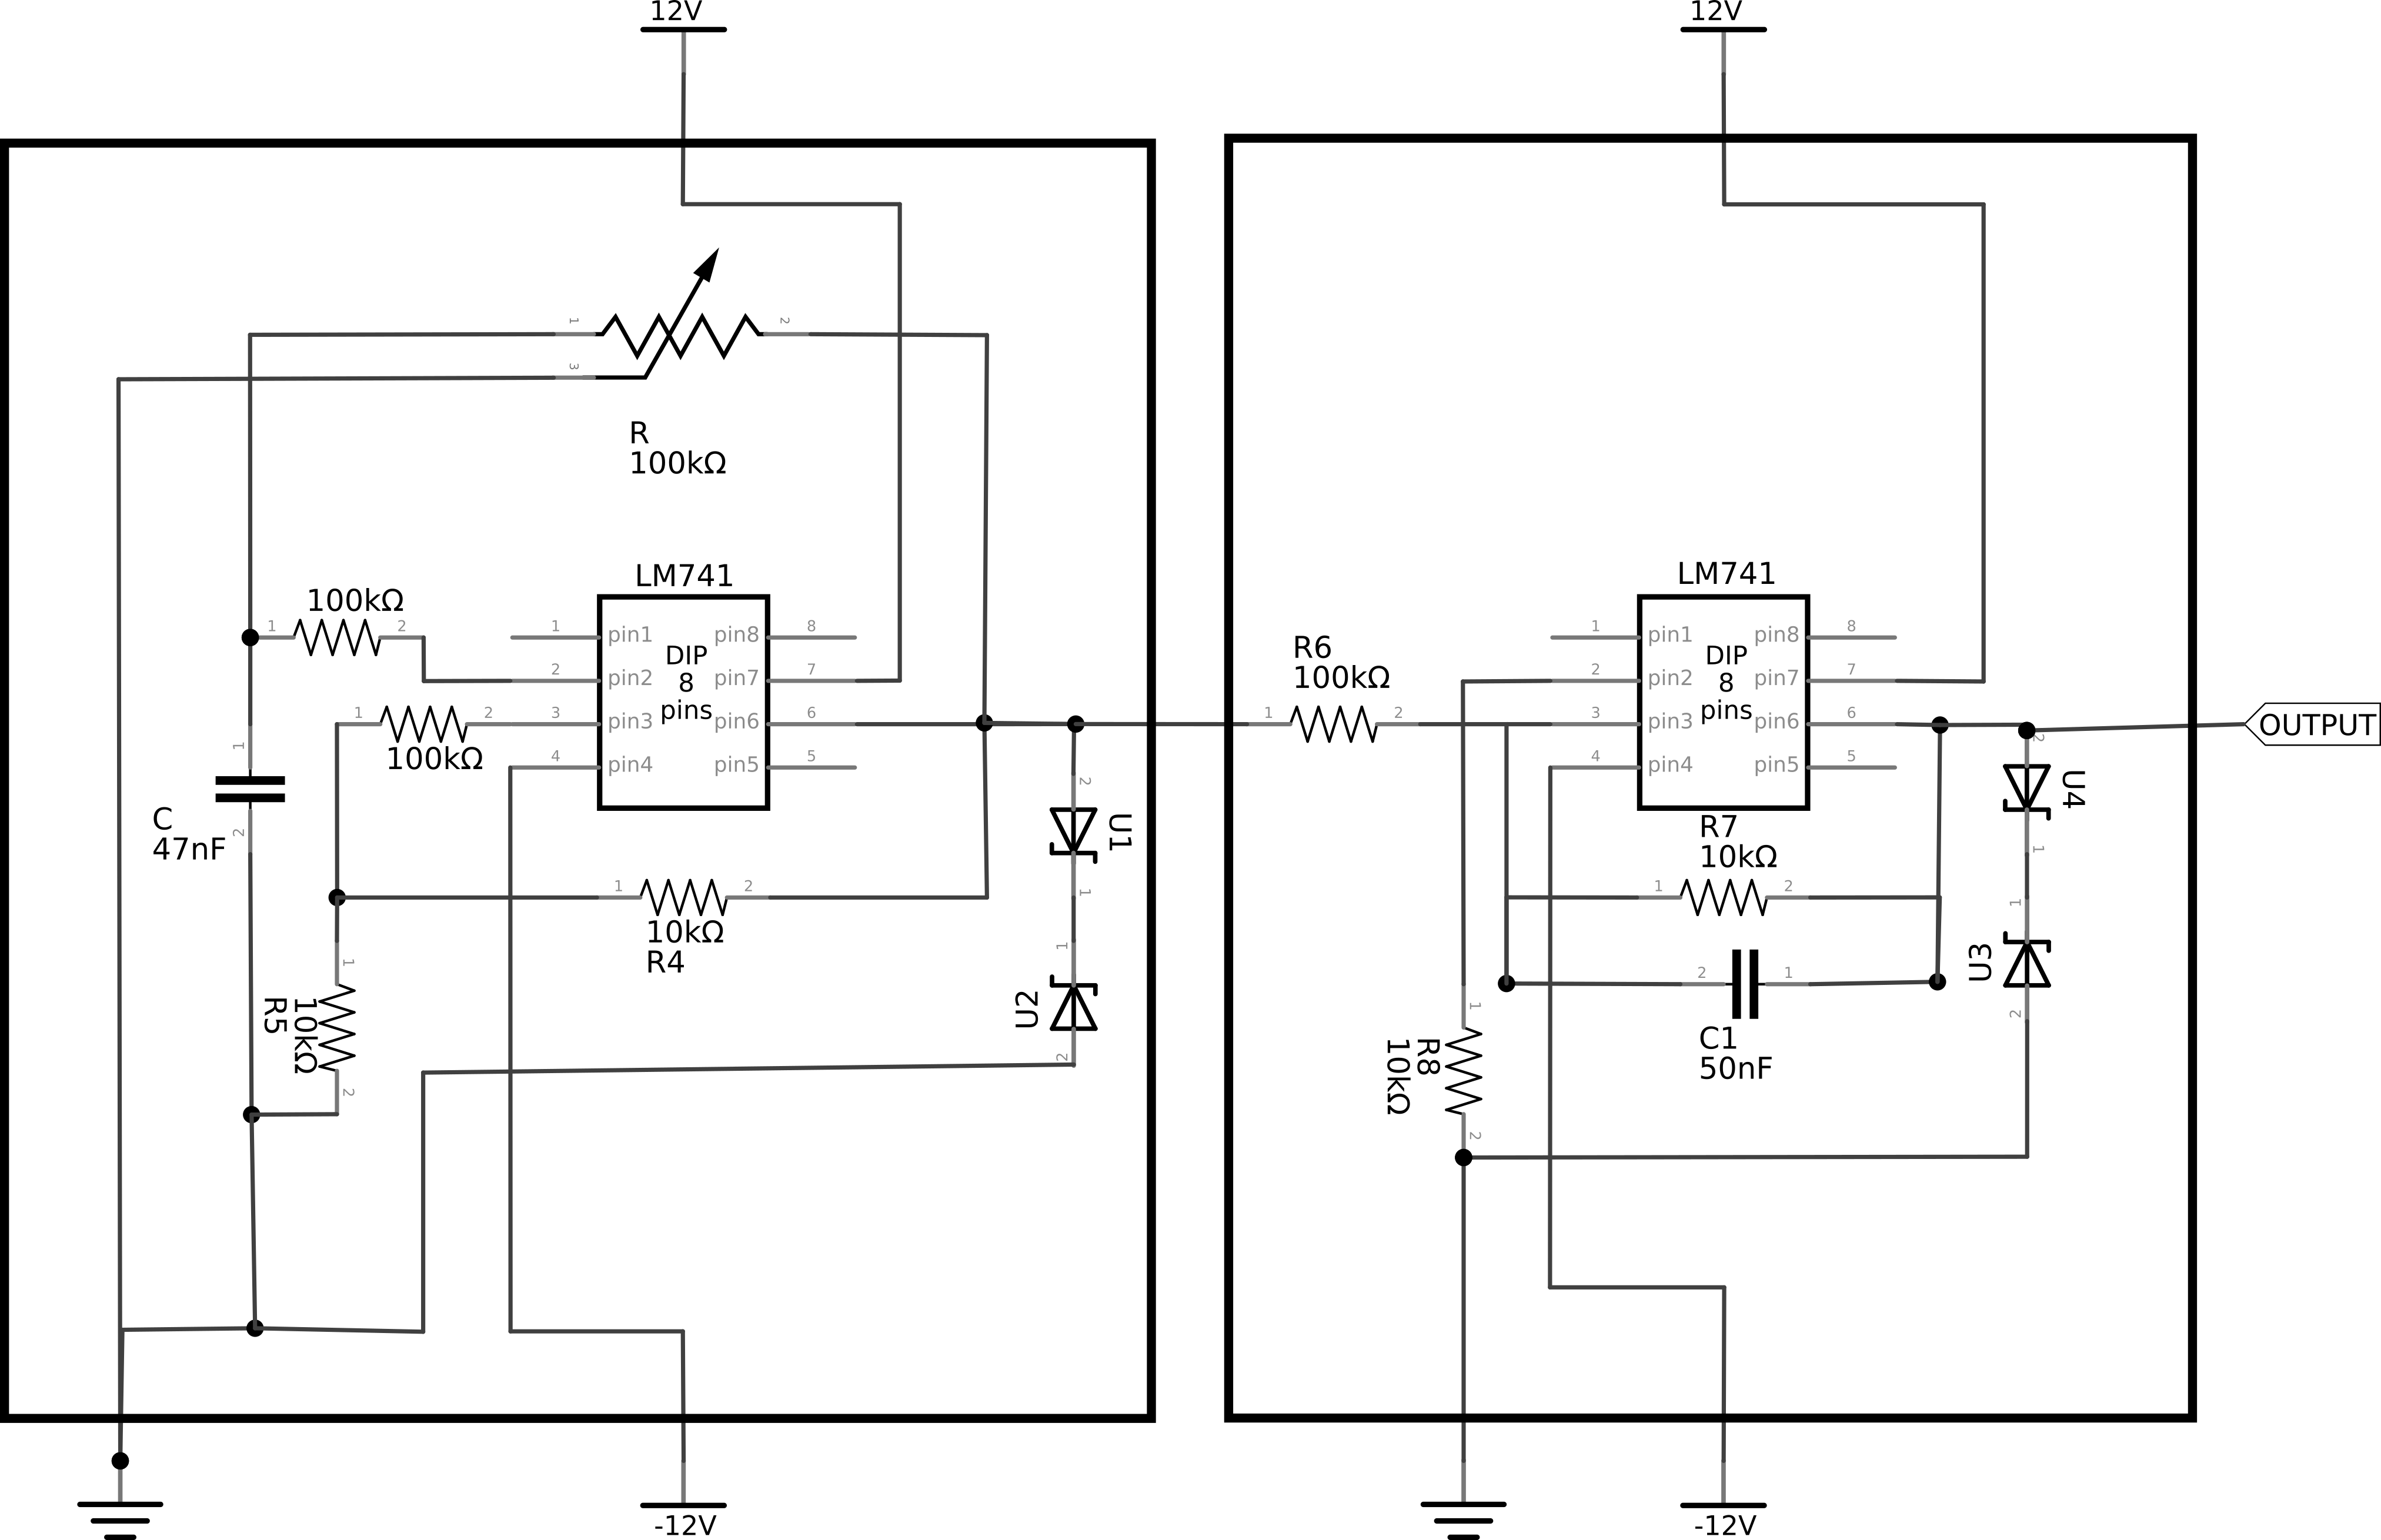
\includegraphics[width=0.95\textwidth]{imgs/triangreal.png}
    \caption{block 3: triangluar wave generator}
\end{figure}

Here, \(R_{4}\) have to be \(10R_{3}\). Frequency is give by same relation as block 2.


\section{connection and switching}
\label{sec:org21b1e01}

For connection of all this block we have used push pull button with two poles. One for power controlling and other for output controlling. Basic diagram of this switch is drawn in figure below.

When switch is \textbf{\textbf{ON}} (means pushed) it will connect 1 terminals with common and complete the circuit. When switch is \textbf{\textbf{OFF}} (pulled condition), the circuit will open and we will not get connection.

\begin{figure}[H]
    \centering
    \label{switchon}
    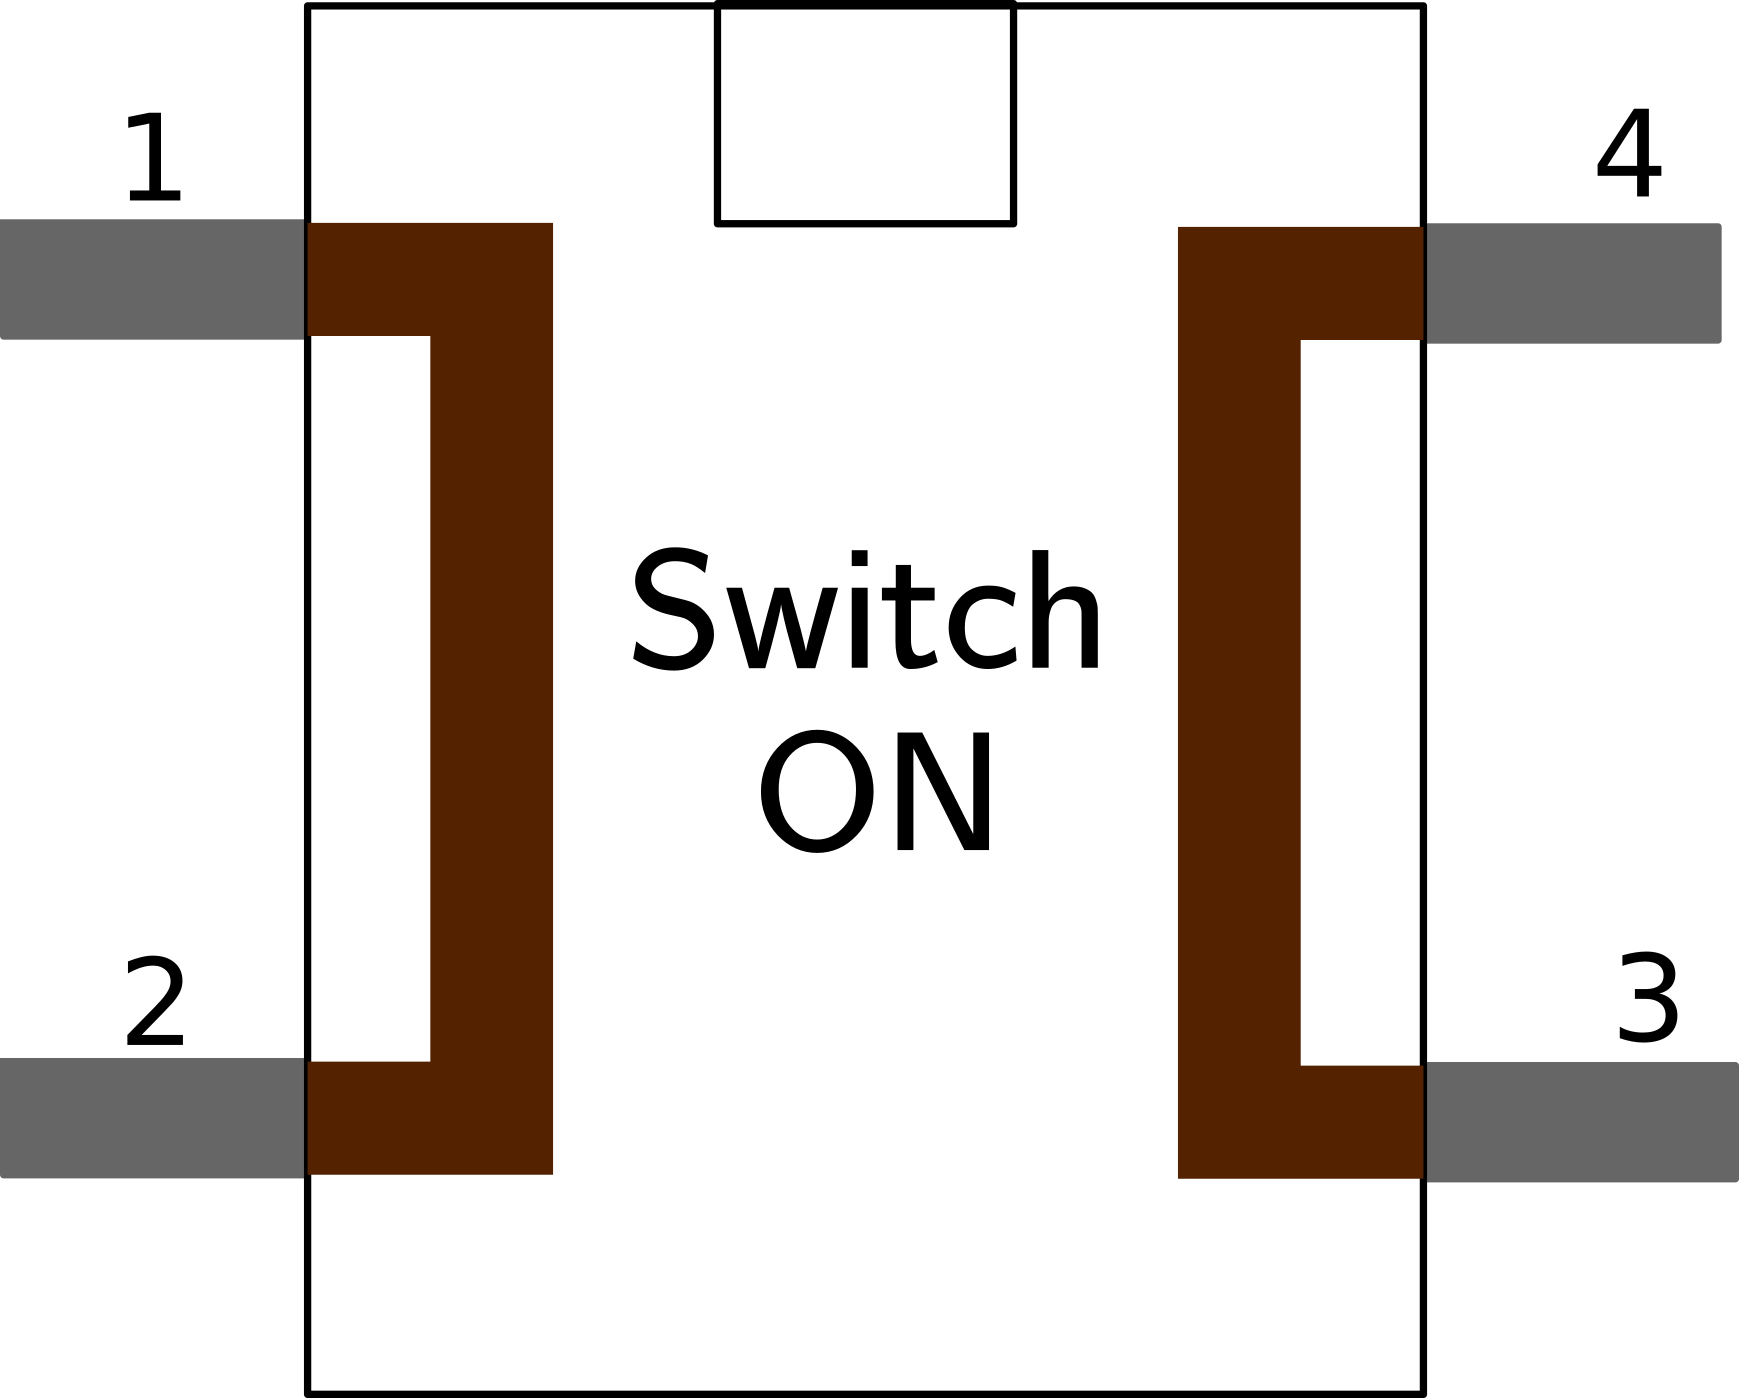
\includegraphics[width=0.5\textwidth]{imgs/switchon.png}
    \caption{switch on state for two pole push button switch}
\end{figure}

\begin{figure}[H]
    \centering
    \label{switchoff}
    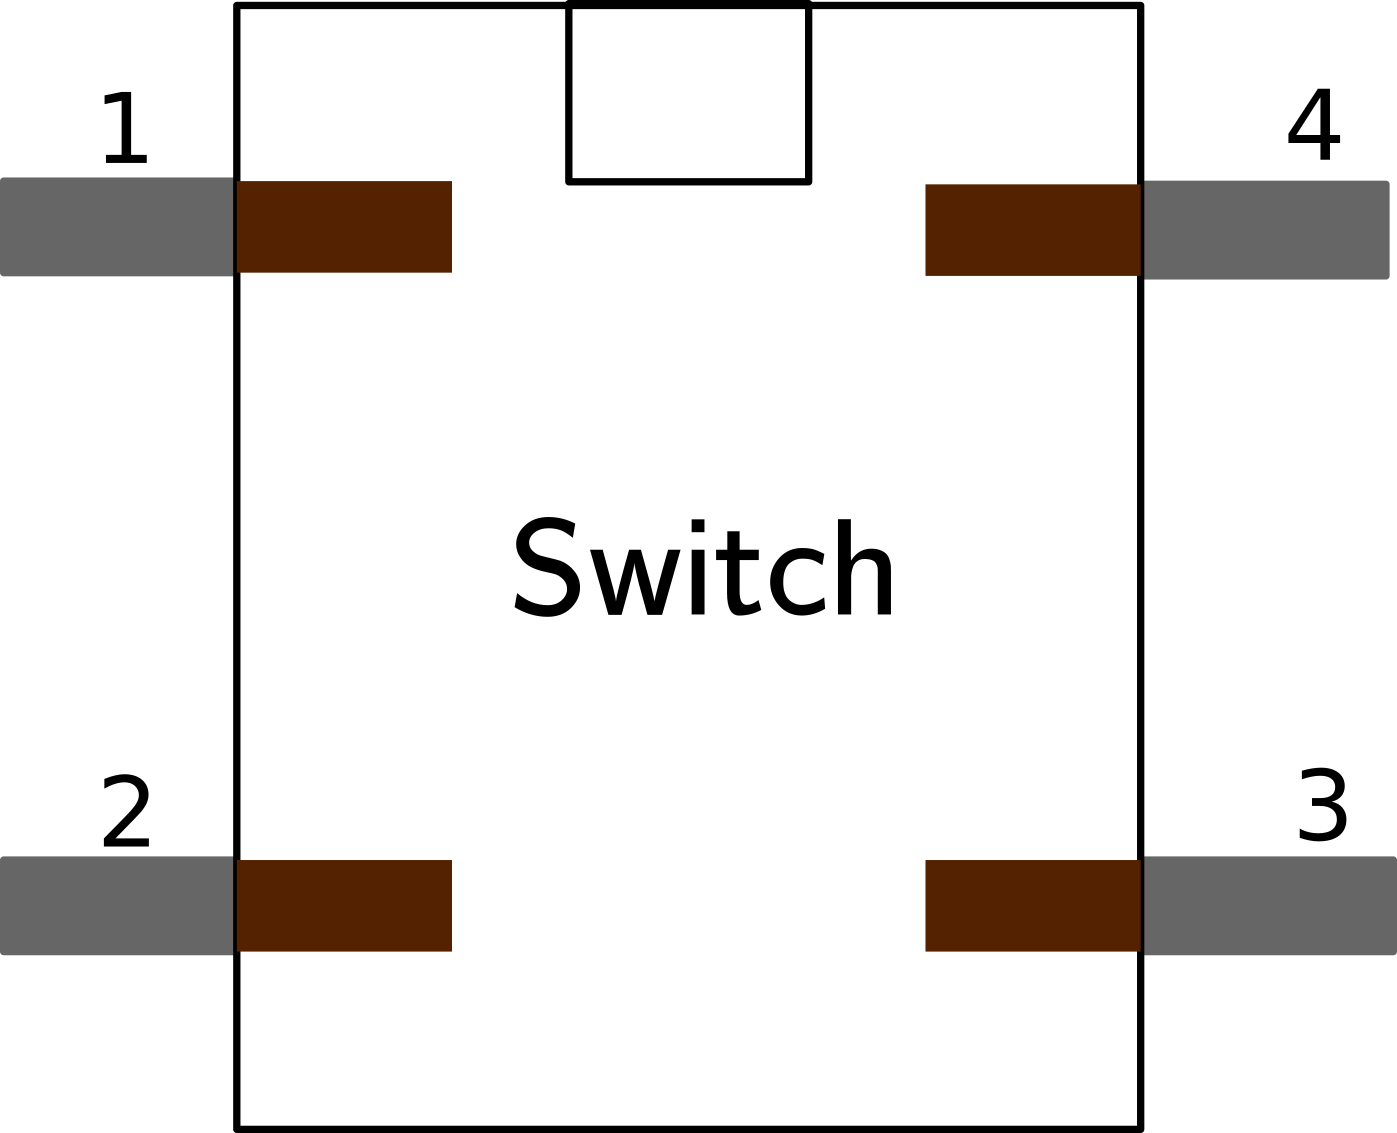
\includegraphics[width=0.5\textwidth]{imgs/switchoff.png}
    \caption{switch off state for two pole push button switch}
\end{figure}

The +Vcc in common (upper common) is completely independent of Output terminal common (lower common). Which means switch can completely operate two tasks, which is when on it power the block and take output and give to CRO. You can see this is on block diagram in figure 1 \label{orgb1d7515}.



\section{Output}
\label{sec:orgdf73c47}

The output of whole circuit which is single output after connecting switches, will goes to CRO (cathode ray oscilloscope), which will measure gain and show signal form.

Theoritically, it shoult give exact signal but errors from ICs, connections, components are reasonable. We are tried our best to minimize it with simulation in Pspice simulations. But real life and simulations are distanced things. We are expected to see some divergence.

\section{Pspice simulations}
\label{sec:org4550a37}

We did Pspice simulation In \url{https://www.falstad.com/circuit/} \cite{Falsted} by Paul Falsted. Here are simlations result from different blocks. This outputs are for Potentiometer valued at \(3.3k\Omega\). We gain peek to peek voltage value at \(2.8917V\) for sine wave and \(2.11V\) and \(2.2\) in square wave and triangular wave respectively. This figures are from matplotlib \cite{Hunter:2007}\cite{harris2020array}, since we could not get from falsted. We got accurate p-p voltages.

\begin{figure}[H]
    \centering
    \label{outputs}
    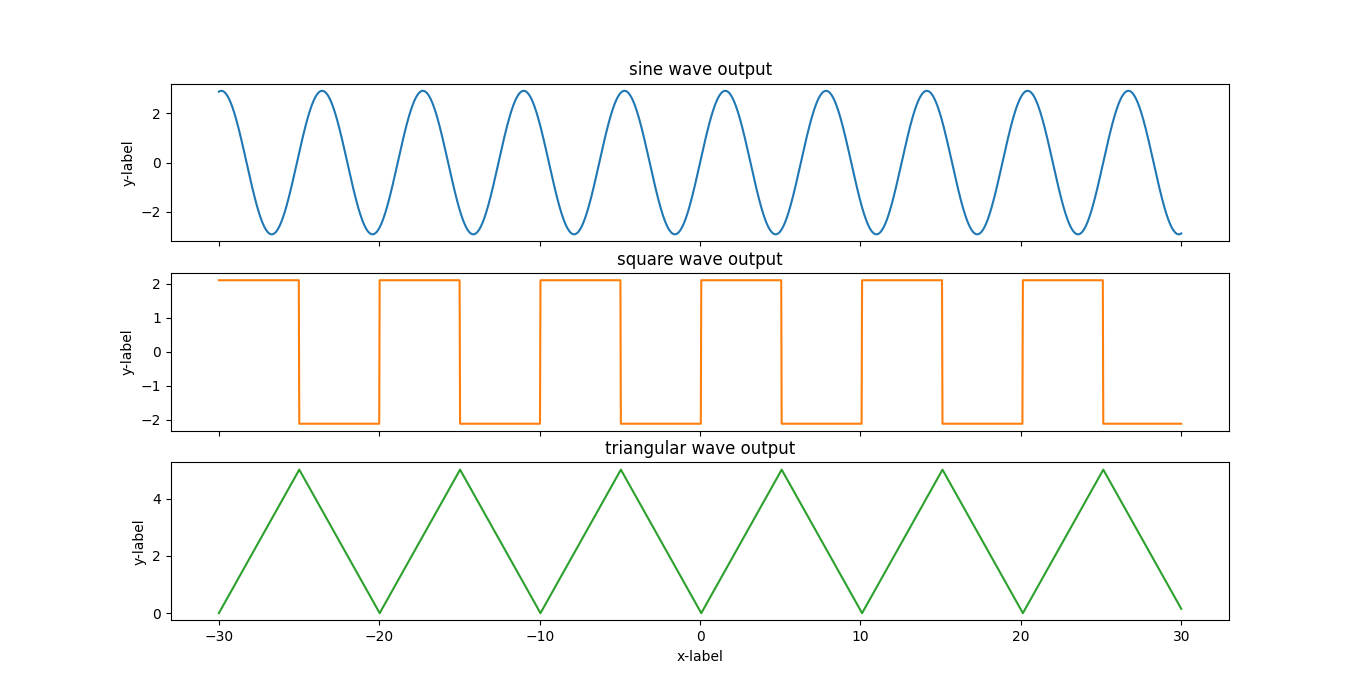
\includegraphics[width=0.8\textwidth]{imgs/outputs.png}
    \caption{Outputs}
\end{figure}


\bibliography{documentation}
\addcontentsline{toc}{section}{References}
\bibliographystyle{plain}
\end{document}
